\subsection{Evaluation of the Extrapolation Error} \label{sec::BGestimation::nonClosure_kineExtp}
Although the good modeling on the extrapolation variables is confirmed in the pre-selection regions, 
the question is whethere they are still good when the signal region selections are applid.
In fact, there is correlation between the well-modeled variables ($\mt$, $\apl$ etc.) and the ill-modeled ones ($\nJetNoGev$, jet transverse momenta, $\meffInc$ etc.) that are not evident at preselection level, however could be addressing in some particular phase space. 
The extrapolation is also affected by the loosened cuts in variables that are already known to be poorly modeled such as MET, so the associated uncertainty needs be quantified. \\

In this sub-section, the extrapolation error is evaluated by injecting an artificial variation in MC compared to the observed MC mis-modeling, and then measure the yield change in a CR and the corresponding SR. Ideally, they show the same response against the injected variation, so that the normalization in CR can perfectly compensate the effect of mis-modeling in SR. Otherwise, the relative difference in their yield variation directly corresponds to the amount of extrapolation error. \\

Figure \ref{fig::BGestimation::valid_extp_2J} - \ref{fig::BGestimation::valid_extp_3B} present the results where the $\wjets$ and $\ttbar$ MC are varied by reweighting the events with:
\begin{align}
 w & = 1 - x \times (\nJetNoGev-2), \mbox{\phantom{MMMM}}\,\,\,\,\,\, x \in [0,0.18]  \mbox{\phantom{MMMM}} (\wjets) \nn  \\
 w & = 1 - x \,\times p_T(\ttbar)/100\gev, \,\,\,\,\,\,\,\,           x \in [0,0.09]  \mbox{\phantom{MMMM}} (\ttbar),
\label{eq::BGestimation::injected_MCvariation}
\end{align}
respectively. The vertical axis on the top panels show the amount of relative change that CR or SR experience by the injected MC variation as a function of $x$. The relative variation in CR (orange) compares to the normalization factor actually obtained via the fit to data, while that in SR (blue) to the ideal normalization factor need to fully correct the SR. The bottom panel display the ratio, namely the resultant extrapolation error. The realistic $x$ is approximately $x_W=0.1$ and $x_{\ttbar}=0.06$ for $\wjets$ and $\ttbar$ respectively, based on the observation of data/MC in Sec. \ref{sec::BGestimation::dataMC} as Eq. (\ref{eq::BGestimation::rwgt_nJ}), (\ref{eq::BGestimation::rwgt_ttPt}) and (\ref{eq::BGestimation::rwgt_ttPt3B}). B-tagging requirement is removed to maintain sufficient statistics, assuming the kinematics are invariant with it. For the $\ttbar$ process, component estimated by the object replacement method is excluded from the test. The extrapolation error from CRs to corresponding VRs are shown in Appendix Sec.\ref{sec::App::valid_extp_VR}. \\

Observed extrapolation error is generally small, which stays within 10$\%$ (20$\%$) for $\wjets$ ($\ttbar$) at the reference magnitude of mis-modeling ($x_W=0.1, \,\,\, x_{\ttbar}=0.06$). These are quoted as systematics error associated with the method in the fit, which is summarized in Table \ref{tab::Uncertainties::noClosure_kineExtp} of Sec. \ref{sec::Uncertainties::nonClosure}. \\

%
% note that このtestはmt/apl extraplationで最大のIssueであるjetのMis-modelingがどれくらい解消できるかというtestであり、本質的にmt spectraとmis-modelingがどれくらい相関しているかを見ているにすぎない。
%in other preselectionにおけるmtの記述が完璧だとした場合にjet selectionかけたときにどれくらいmt. aplの分布がズレるかというtestである. 
% 
%このtestでevaluateしたerrorは手法に由来するsystematicとしてassignするが、jet以外の要因によるMT spectraのvariationは別個評価する必要がある. (instrumental, theory etc.)
%これらは7章でevaluateする

Note that this check is only quantifying the error in the methodology; how much the MC mis-modeling in terms of jet activities can be corrected if the other MC description is perfect.
In reality, the shape of $\mt$ or $\apl$ distribution can be varies by the other reasons, and the uncertainties have to be assigned additionally. This will be discussed in Sec. \ref{sec::Uncertainties}.

\clearpage
%\begin{figure}[h]
  \centering
    \subfig{0.48}{figures/BGestimation/valid_extp/SFTF_Wjets_Preselection_meff1500_extp_mt__nJet30.pdf}{}
    \subfig{0.48}{figures/BGestimation/valid_extp/SFTF_Wjets_Preselection_meff1500_extp_LepAplanarity__nJet30.pdf}{}
    \caption{ Closure error for $\wjets$ process by the extrapolation using (a) $\mt$ (b) $\apl$ as function of the magnitude of injected linear mis-modeling on $\nJet$: $y_{\ttbar} = 1.0 - x \times \nJet)$. All evaluated by MC.   \label{fig::BGestimation::valid_extp1} }
\end{figure}

%%%%%%%%%%%%%%%%
\begin{figure}[h]
  \centering
    \subfig{0.48}{figures/BGestimation/valid_extp/SFTF_Wjets_Preselection_meff1500_extp_mt__WPt.pdf}{}
    \subfig{0.48}{figures/BGestimation/valid_extp/SFTF_Wjets_Preselection_meff1500_extp_LepAplanarity__WPt.pdf}{}
    \caption{ Closure error for $\wjets$ process by the extrapolation using (a) $\mt$ (b) $\apl$ as function of the magnitude of injected linear mis-modeling on $\nJet$: $y_{\ttbar} = 1.0 - x \times \nJet)$. All evaluated by MC.   \label{fig::BGestimation::valid_extp2} }
\end{figure}


%%%%%%%%%%%%%%%%
\begin{figure}[h]
  \centering
    \subfig{0.48}{figures/BGestimation/valid_extp/SFTF_tt_Preselection_meff1500_extp_mt__ttPt.pdf}{}
    \subfig{0.48}{figures/BGestimation/valid_extp/SFTF_tt_Preselection_meff1500_extp_LepAplanarity__ttPt.pdf}{}
    \caption{ Closure error for $\ttbar$ process by the extrapolation using (a) $\mt$ (b) $\apl$ as function of the magnitude of injected linear mis-modeling on $p_T(\ttbar)$: $y_{\ttbar} = 1.0 - x \times p_T(\ttbar))$. All evaluated by MC.   \label{fig::BGestimation::valid_extp1} }
\end{figure}

%%%%%%%%%%%%%%%%
\begin{figure}[h]
  \centering
    \subfig{0.48}{figures/BGestimation/valid_extp/SFTF_tt_Preselection_meff1500_extp_mt__meff.pdf}{}
    \subfig{0.48}{figures/BGestimation/valid_extp/SFTF_tt_Preselection_meff1500_extp_LepAplanarity__meff.pdf}{}
    \caption{ Closure error for $\ttbar$ process by the extrapolation using (a) $\mt$ (b) $\apl$ as function of the magnitude of injected linear mis-modeling on $meffInc$: $y_{\ttbar} = 1.0 - x \times \meffInc)$. All evaluated by MC.   \label{fig::BGestimation::valid_extp1} }
\end{figure}



%%%%%%%%%%%%%%%% SR2J
\begin{figure}[h]
  \centering
    \subfigure[]{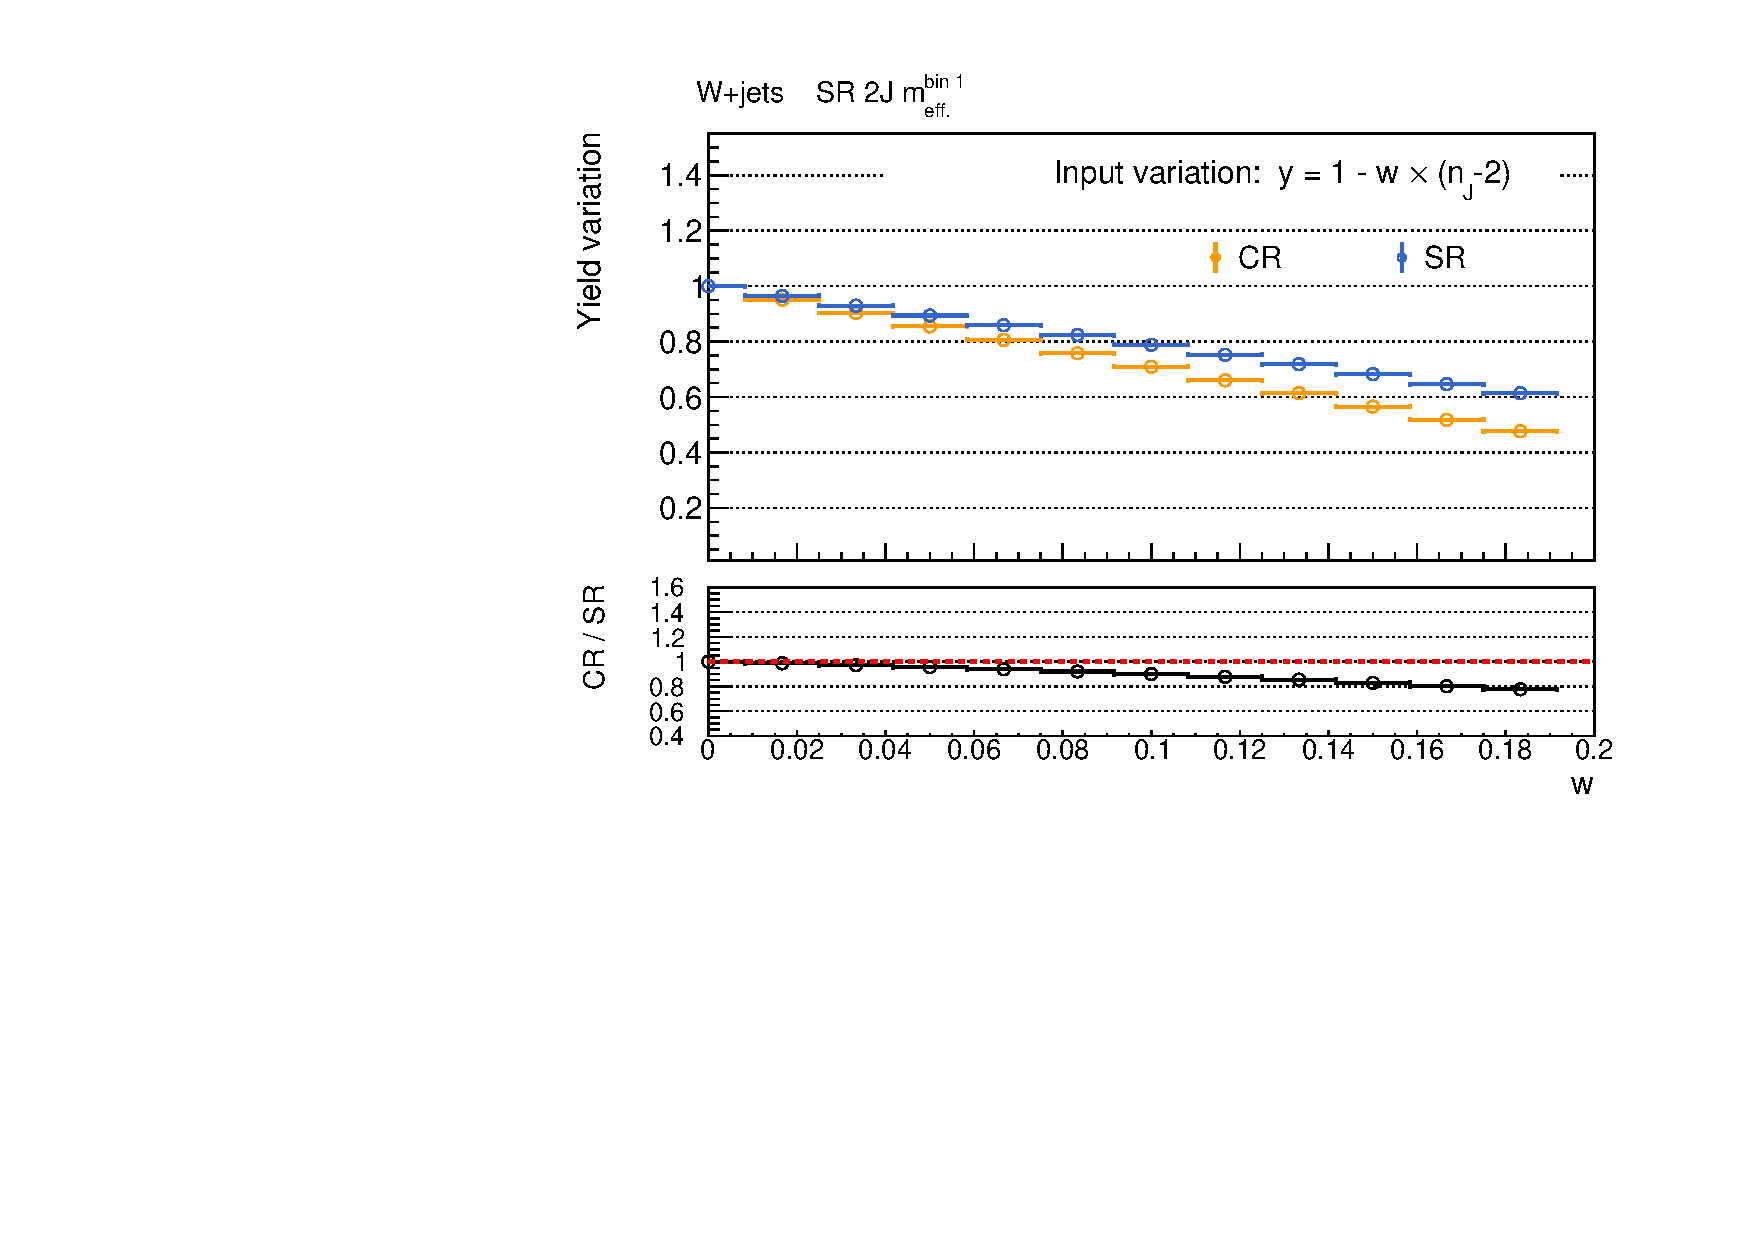
\includegraphics[width=0.488\textwidth]{figures/BGestimation/valid_extp/SFTF_wjets_SR2JMEFF1_extp_var2J__nJet30.pdf}}
    \subfigure[]{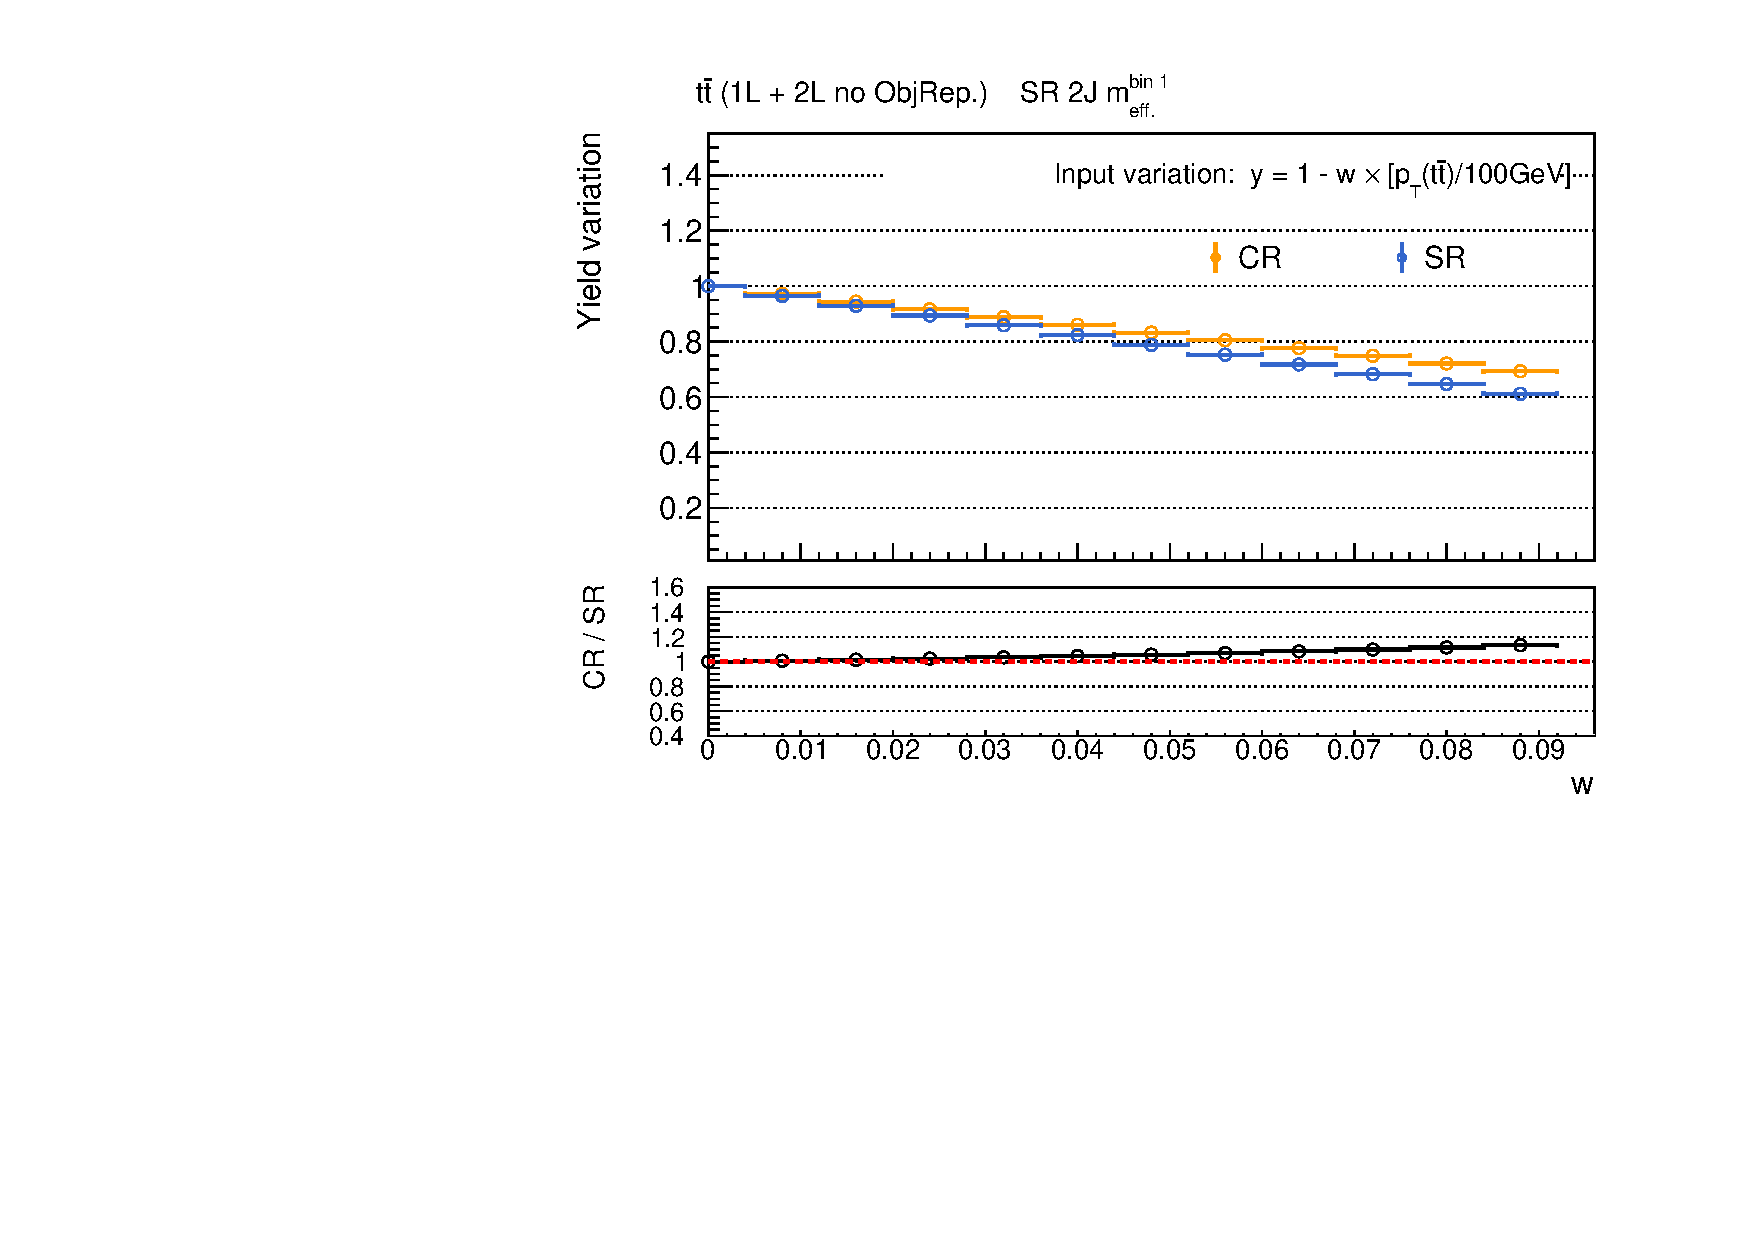
\includegraphics[width=0.488\textwidth]{figures/BGestimation/valid_extp/SFTF_ttNoObjRep_SR2JMEFF1_extp_var2J__ttPt.pdf}}
    \subfigure[]{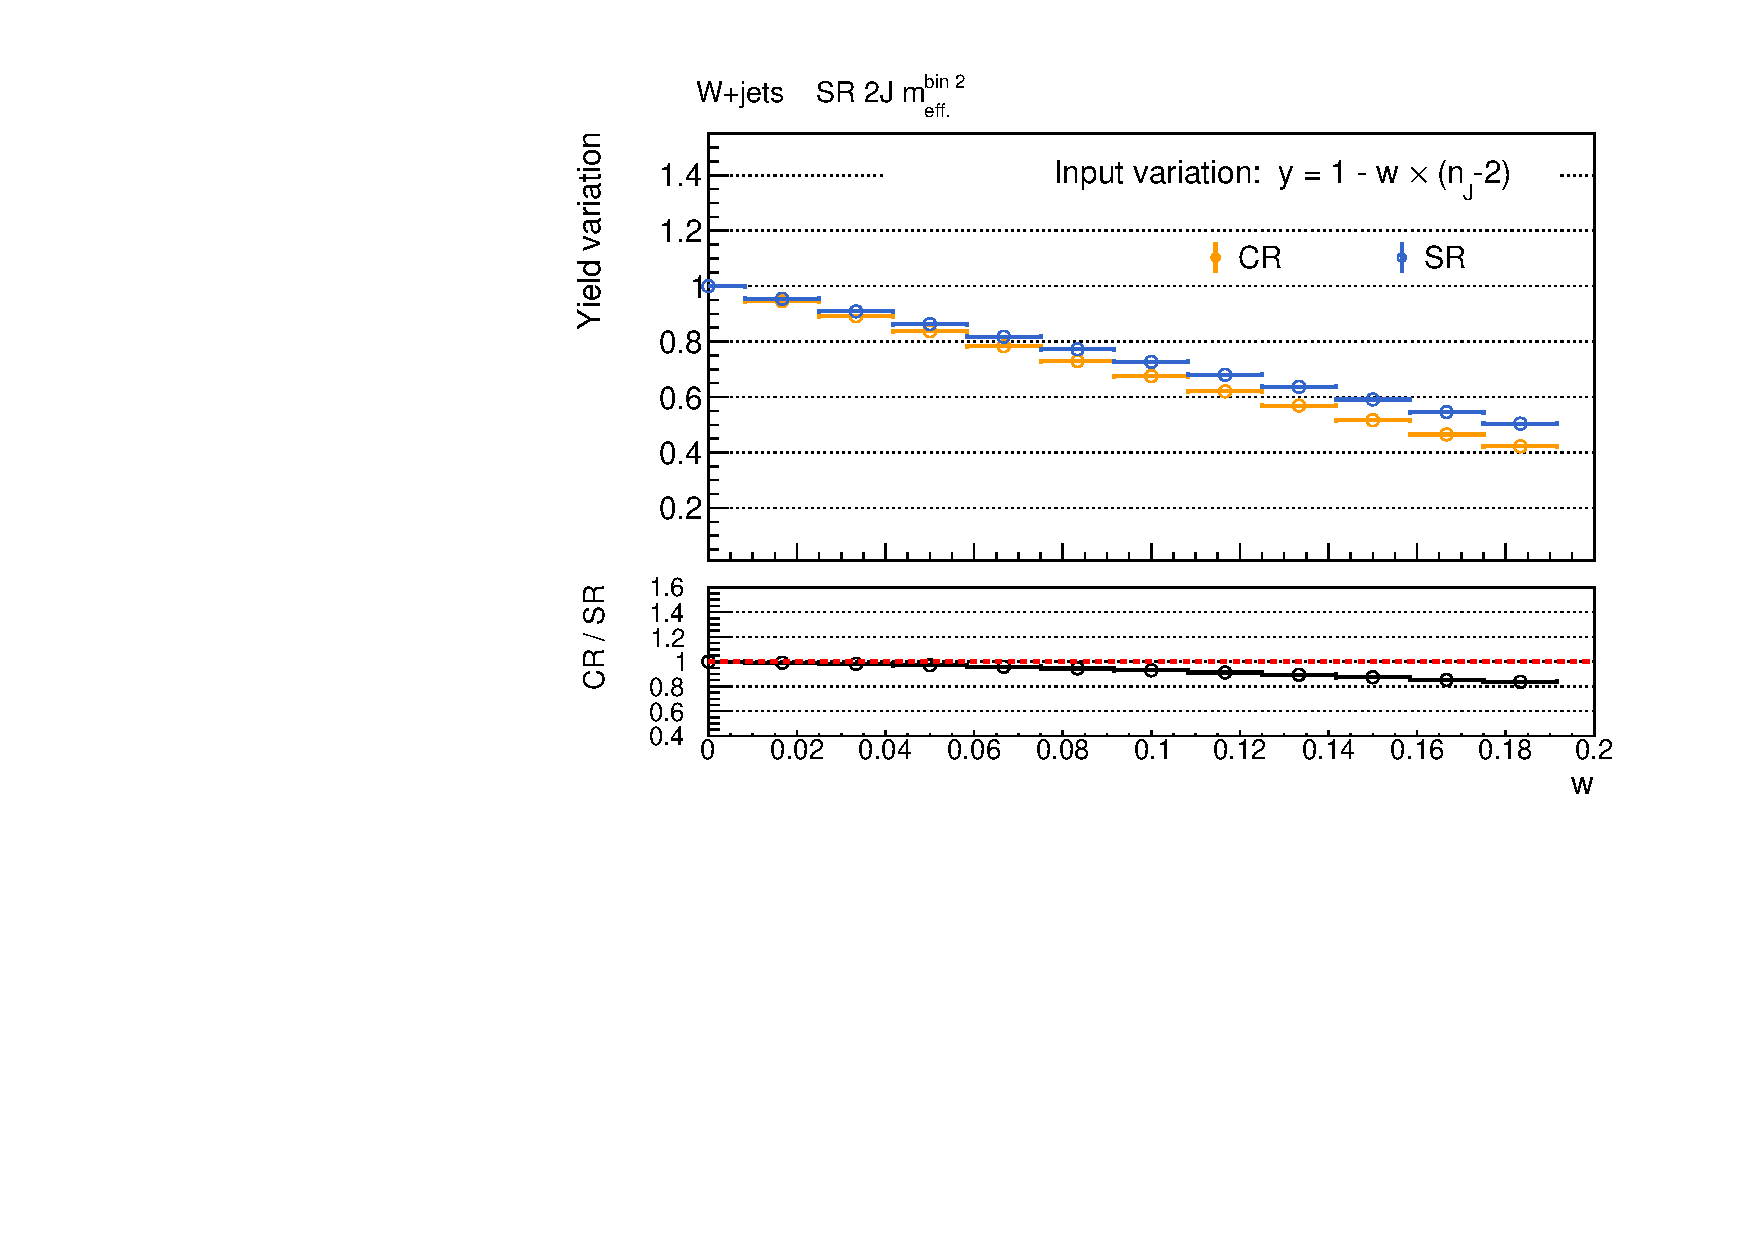
\includegraphics[width=0.488\textwidth]{figures/BGestimation/valid_extp/SFTF_wjets_SR2JMEFF2_extp_var2J__nJet30.pdf}}
    \subfigure[]{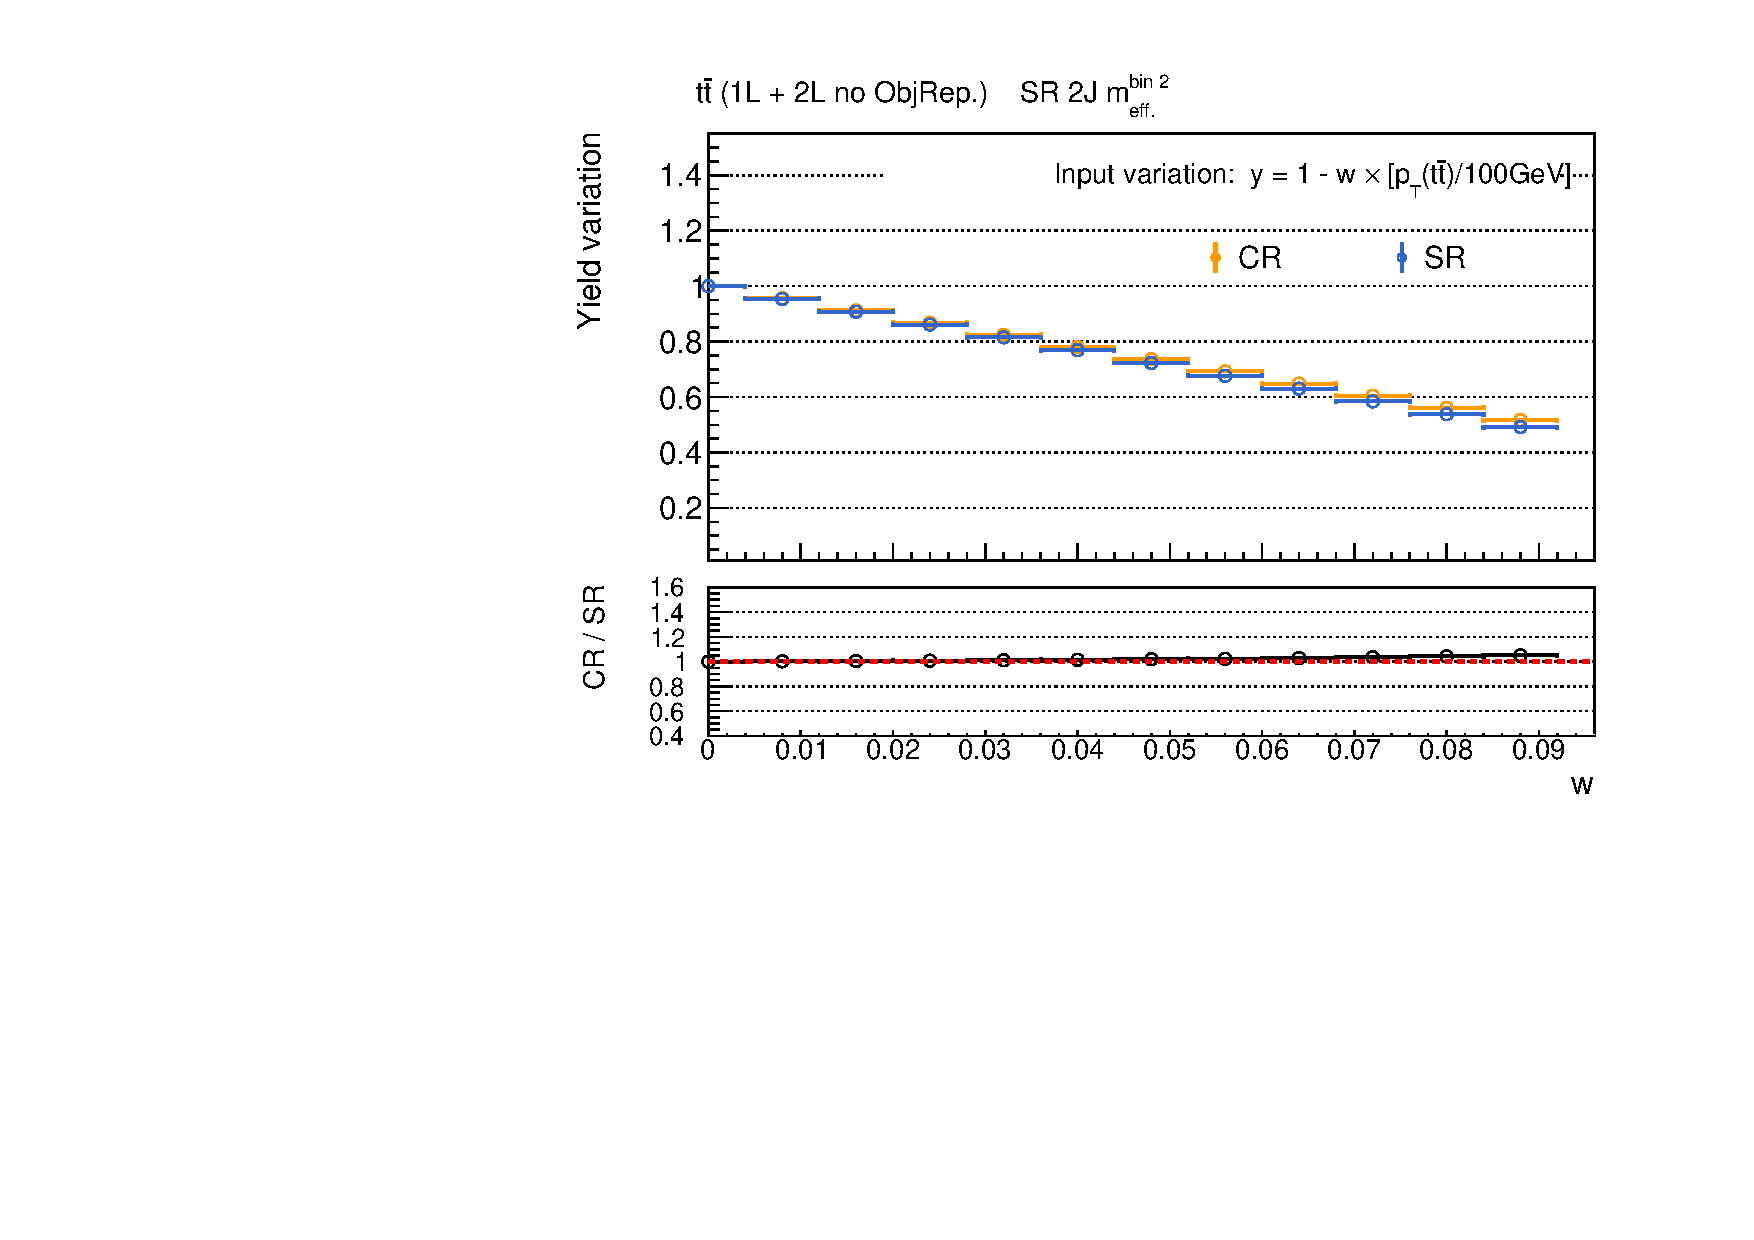
\includegraphics[width=0.488\textwidth]{figures/BGestimation/valid_extp/SFTF_ttNoObjRep_SR2JMEFF2_extp_var2J__ttPt.pdf}}
    \subfigure[]{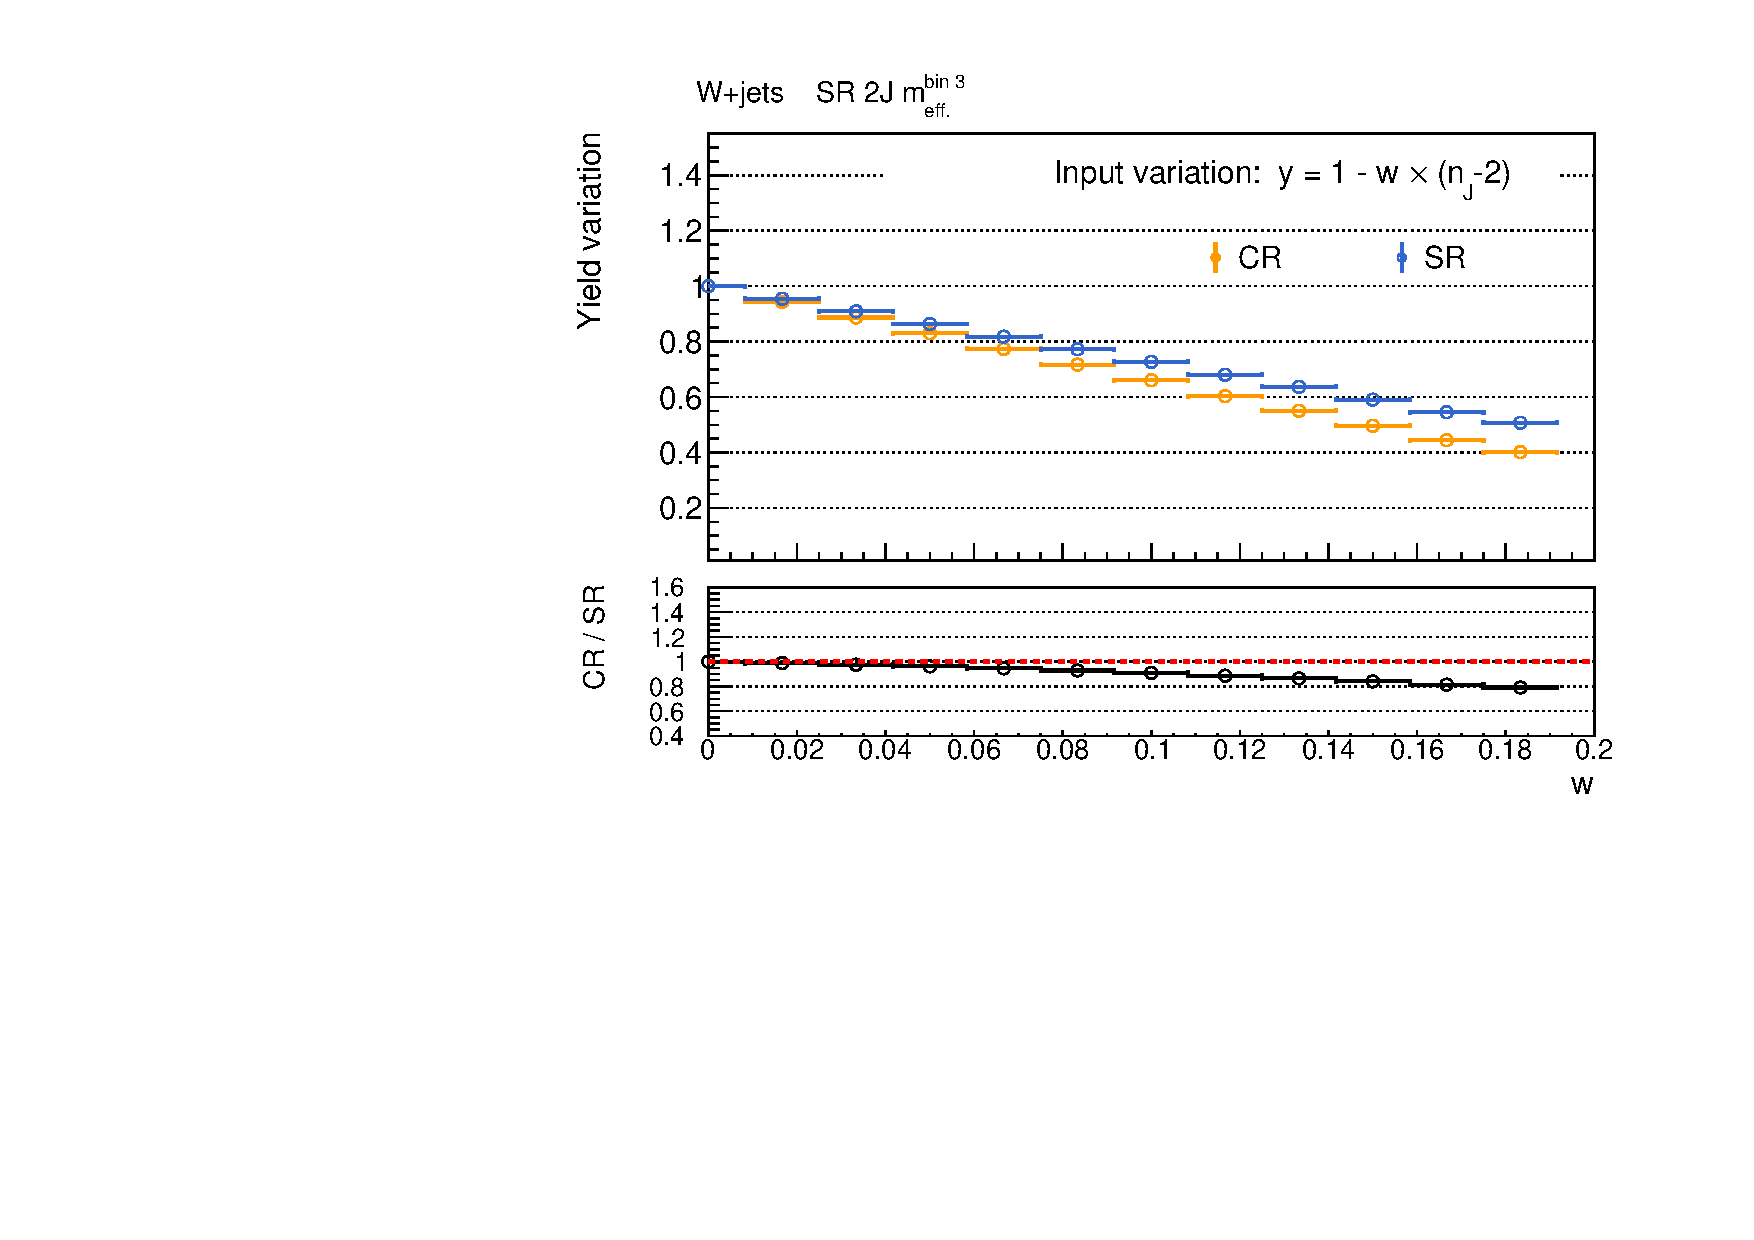
\includegraphics[width=0.488\textwidth]{figures/BGestimation/valid_extp/SFTF_wjets_SR2JMEFF3_extp_var2J__nJet30.pdf}}
    \subfigure[]{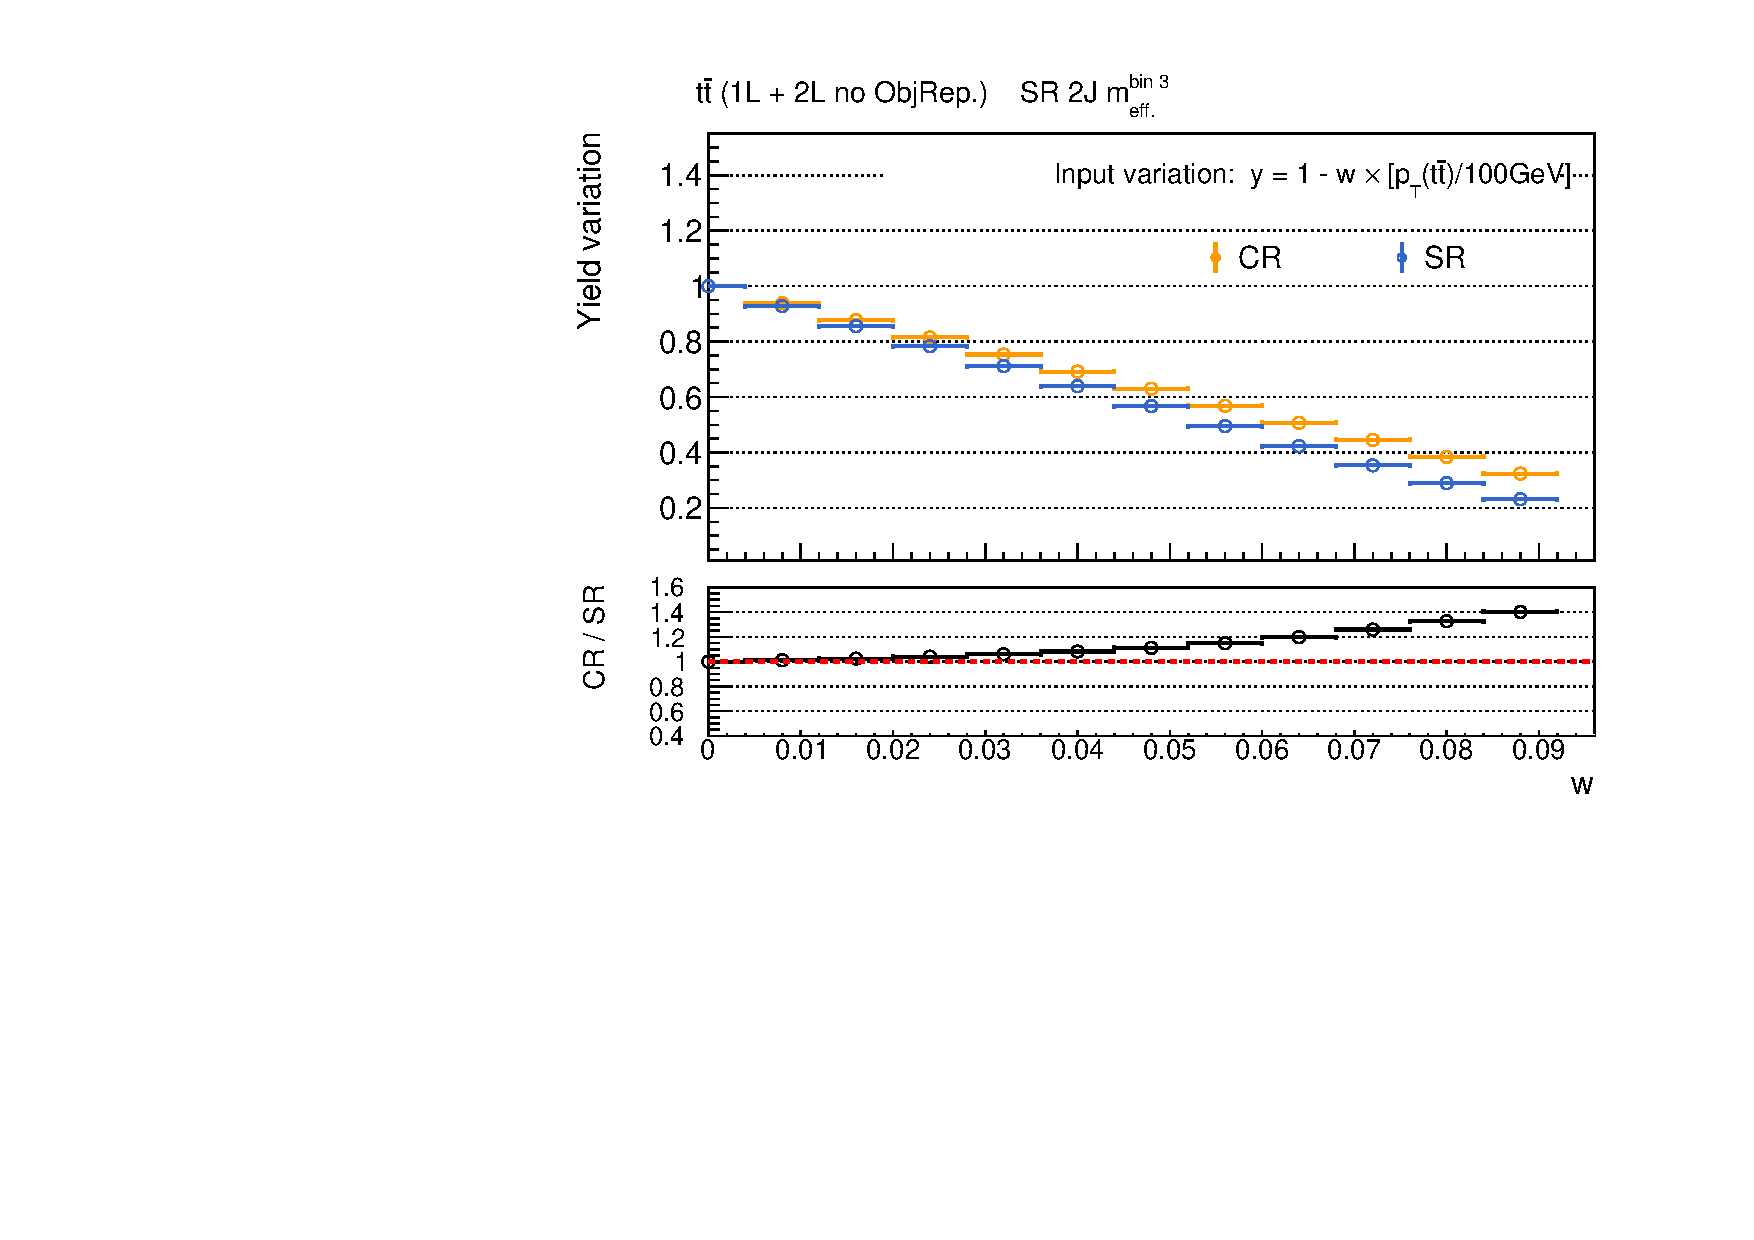
\includegraphics[width=0.488\textwidth]{figures/BGestimation/valid_extp/SFTF_ttNoObjRep_SR2JMEFF3_extp_var2J__ttPt.pdf}}
 \caption{Extrapolation error in SR/CR 2J. B-tagging requirement is removed. Top pannels show the yield variation of (a) $\wjets$ and (b) $\ttbar$ when injecting the variation by reweighting the MC with Eq. \ref{eq::BGestimation::injected_MCvariation}. Bottom rows are the relative difference in their response against the injected variation, namely the extrapolation errir. For the $\ttbar$ process, component estimated by the object replacement method is removed.  \label{fig::BGestimation::valid_extp_2J} }
\end{figure}



%%%%%%%%%%%%%%%% SR6J
\begin{figure}[h]
  \centering
    \subfigure[]{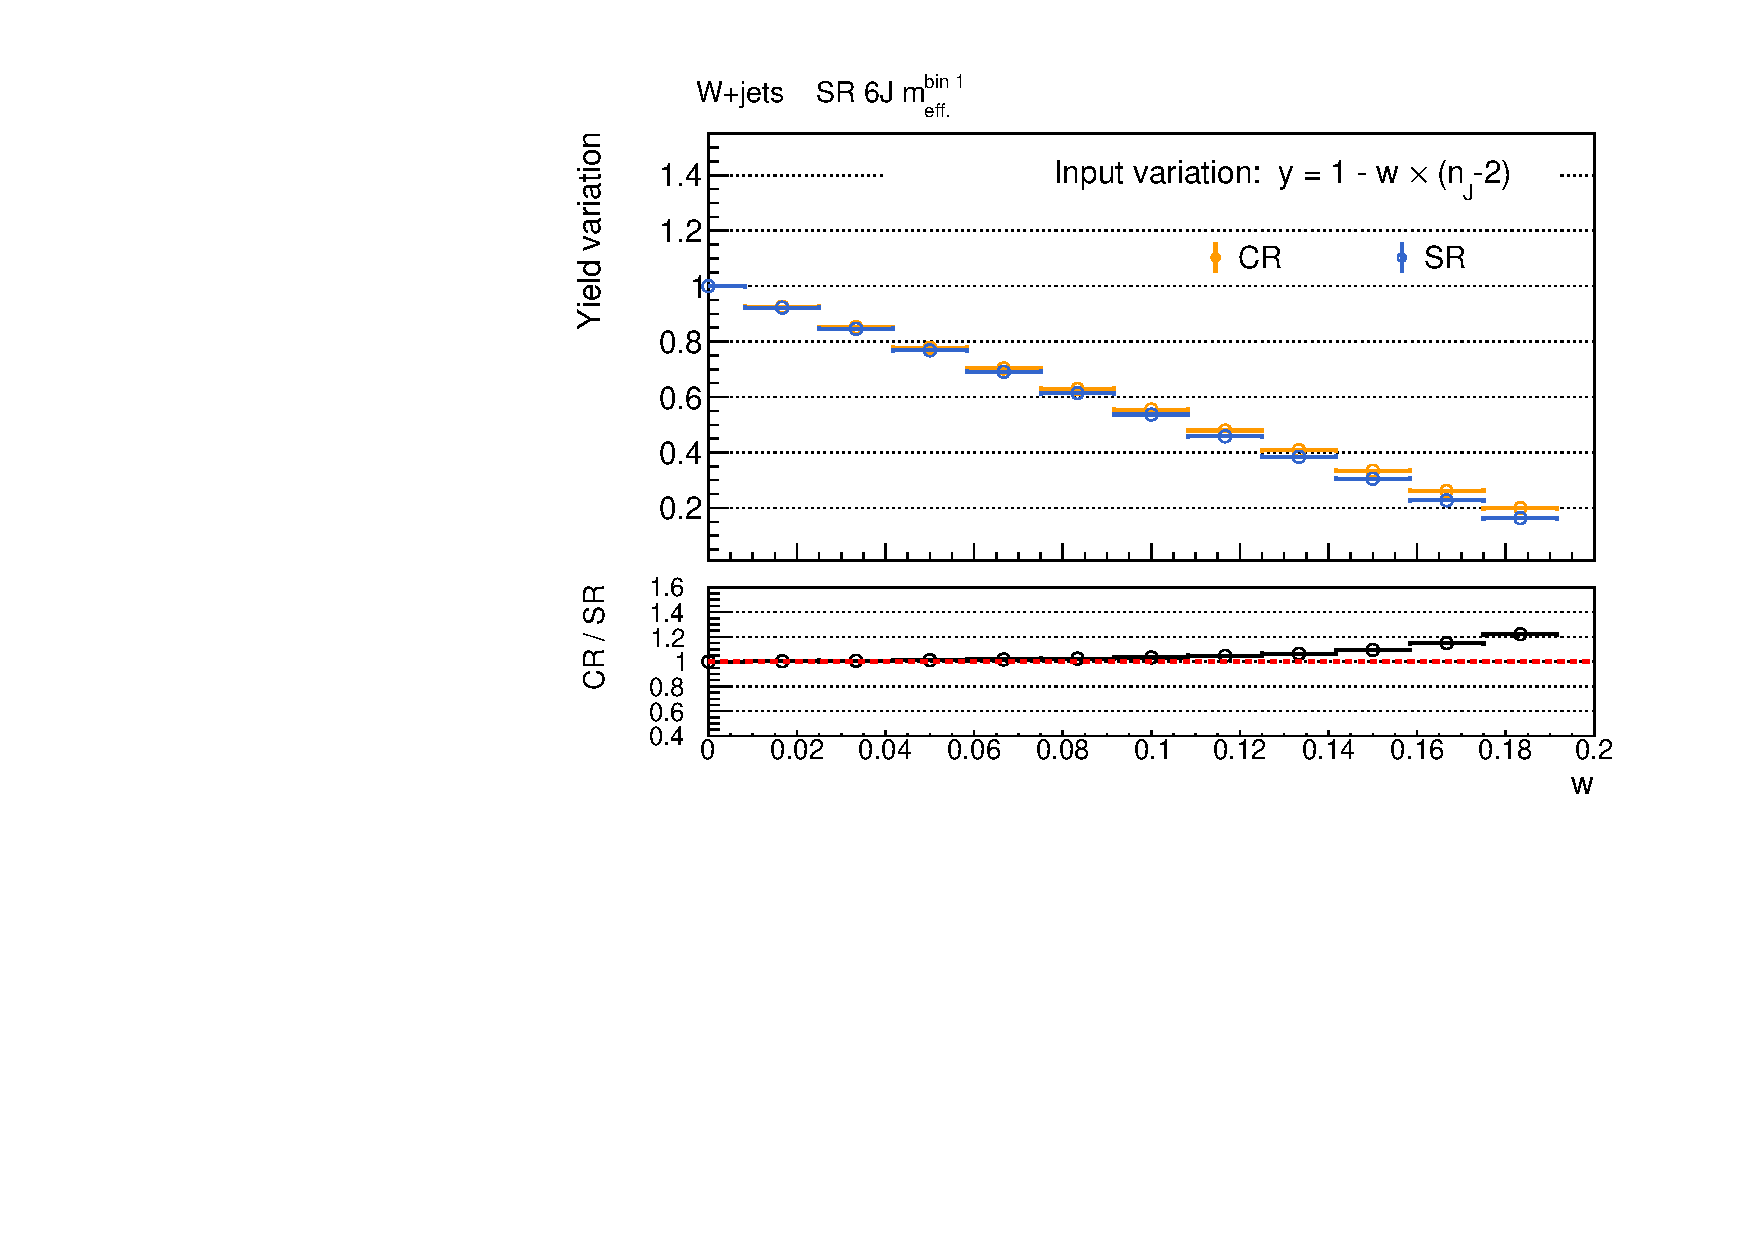
\includegraphics[width=0.488\textwidth]{figures/BGestimation/valid_extp/SFTF_wjets_SR6JMEFF1_extp_var6J__nJet30.pdf}}
    \subfigure[]{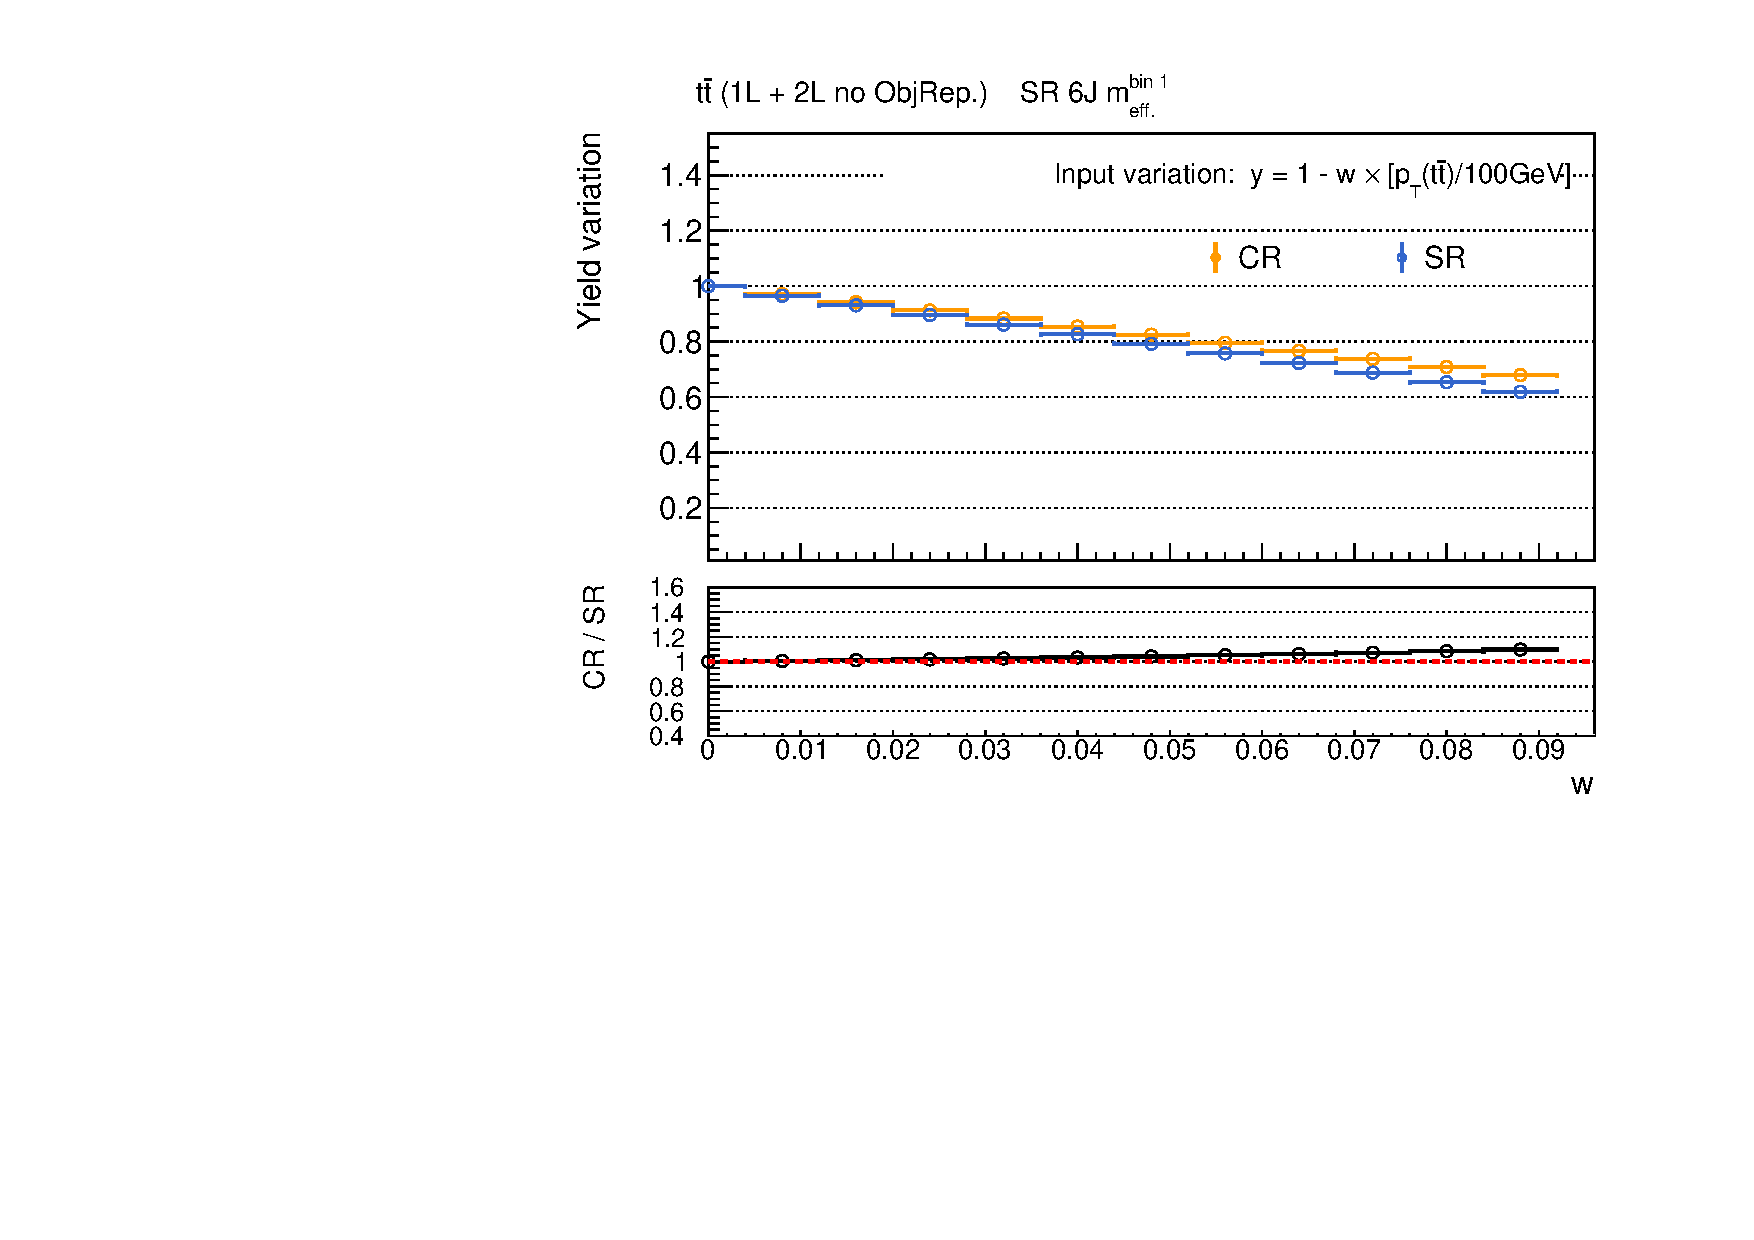
\includegraphics[width=0.488\textwidth]{figures/BGestimation/valid_extp/SFTF_ttNoObjRep_SR6JMEFF1_extp_var6J__ttPt.pdf}}
    \subfigure[]{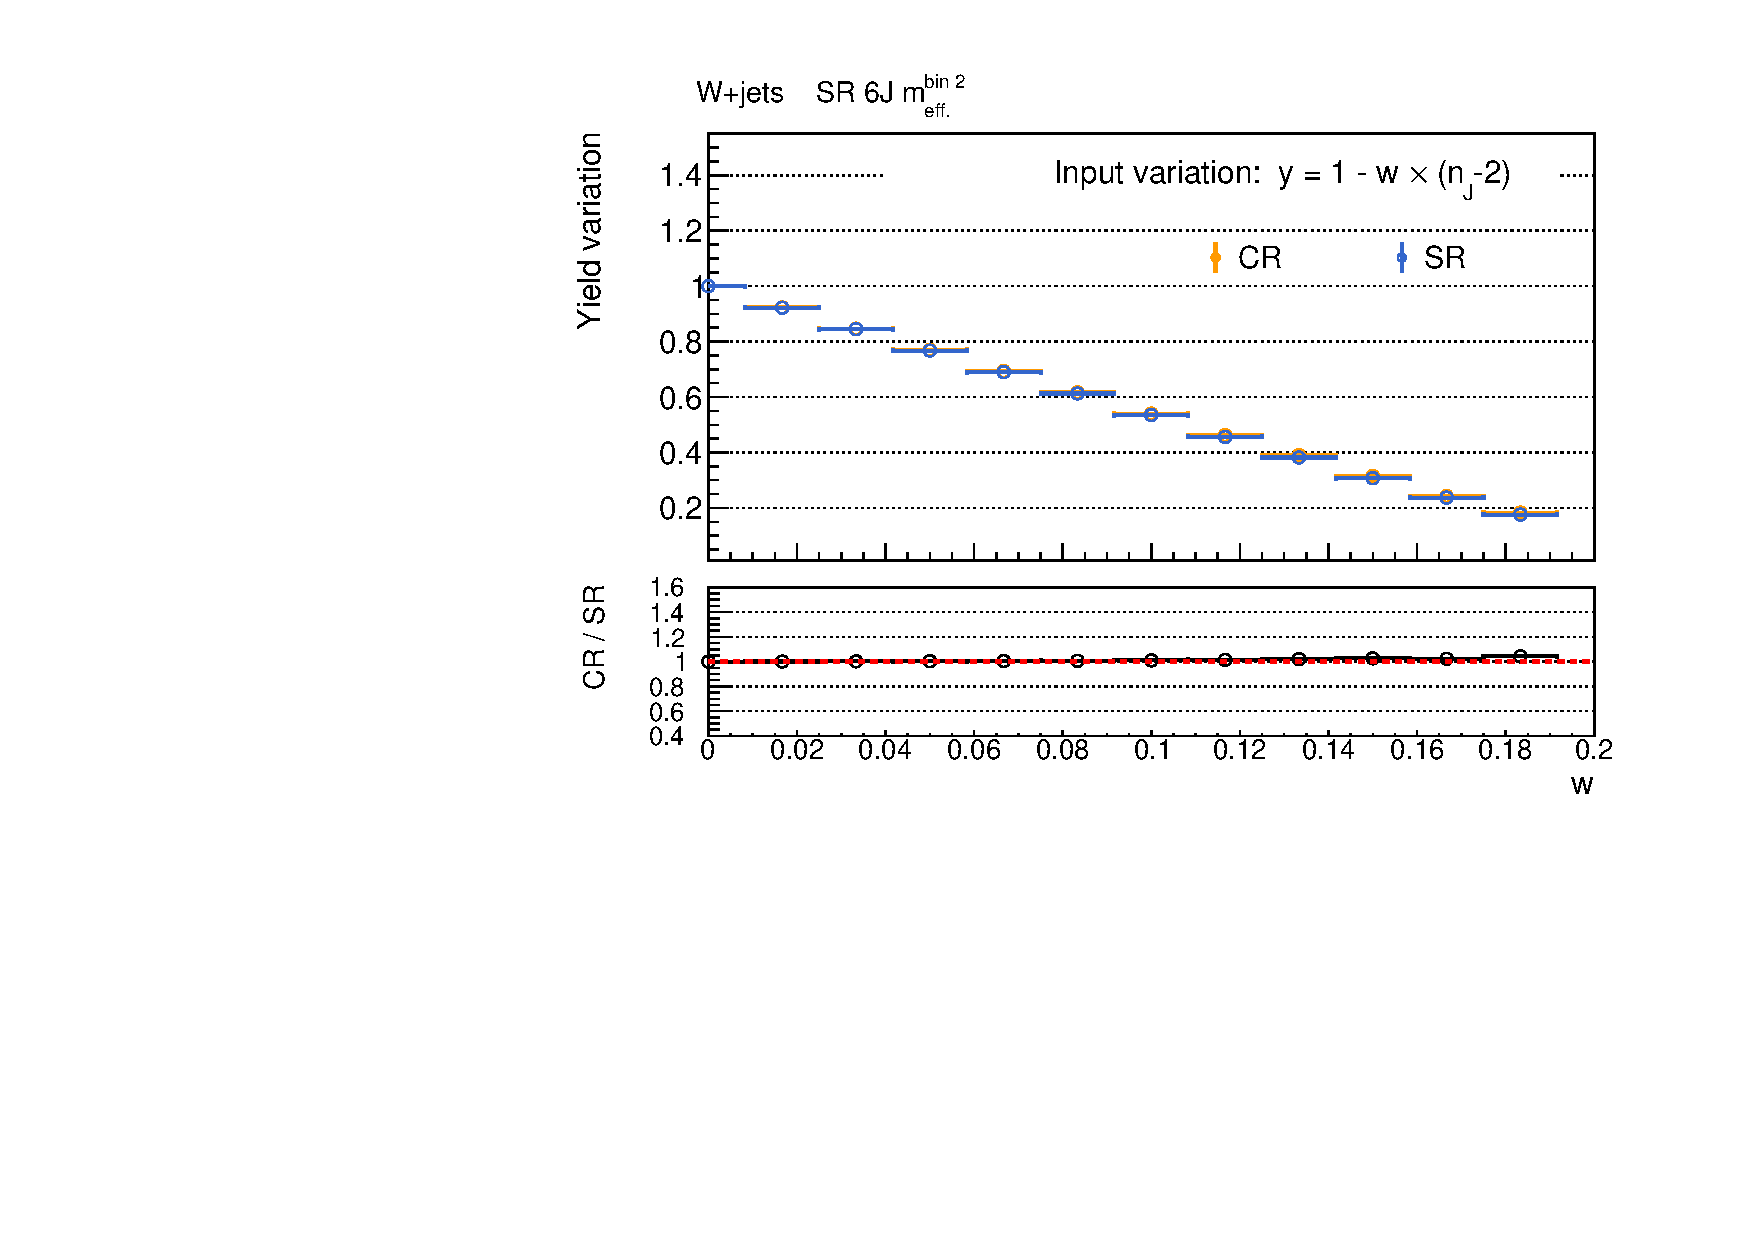
\includegraphics[width=0.488\textwidth]{figures/BGestimation/valid_extp/SFTF_wjets_SR6JMEFF2_extp_var6J__nJet30.pdf}}
    \subfigure[]{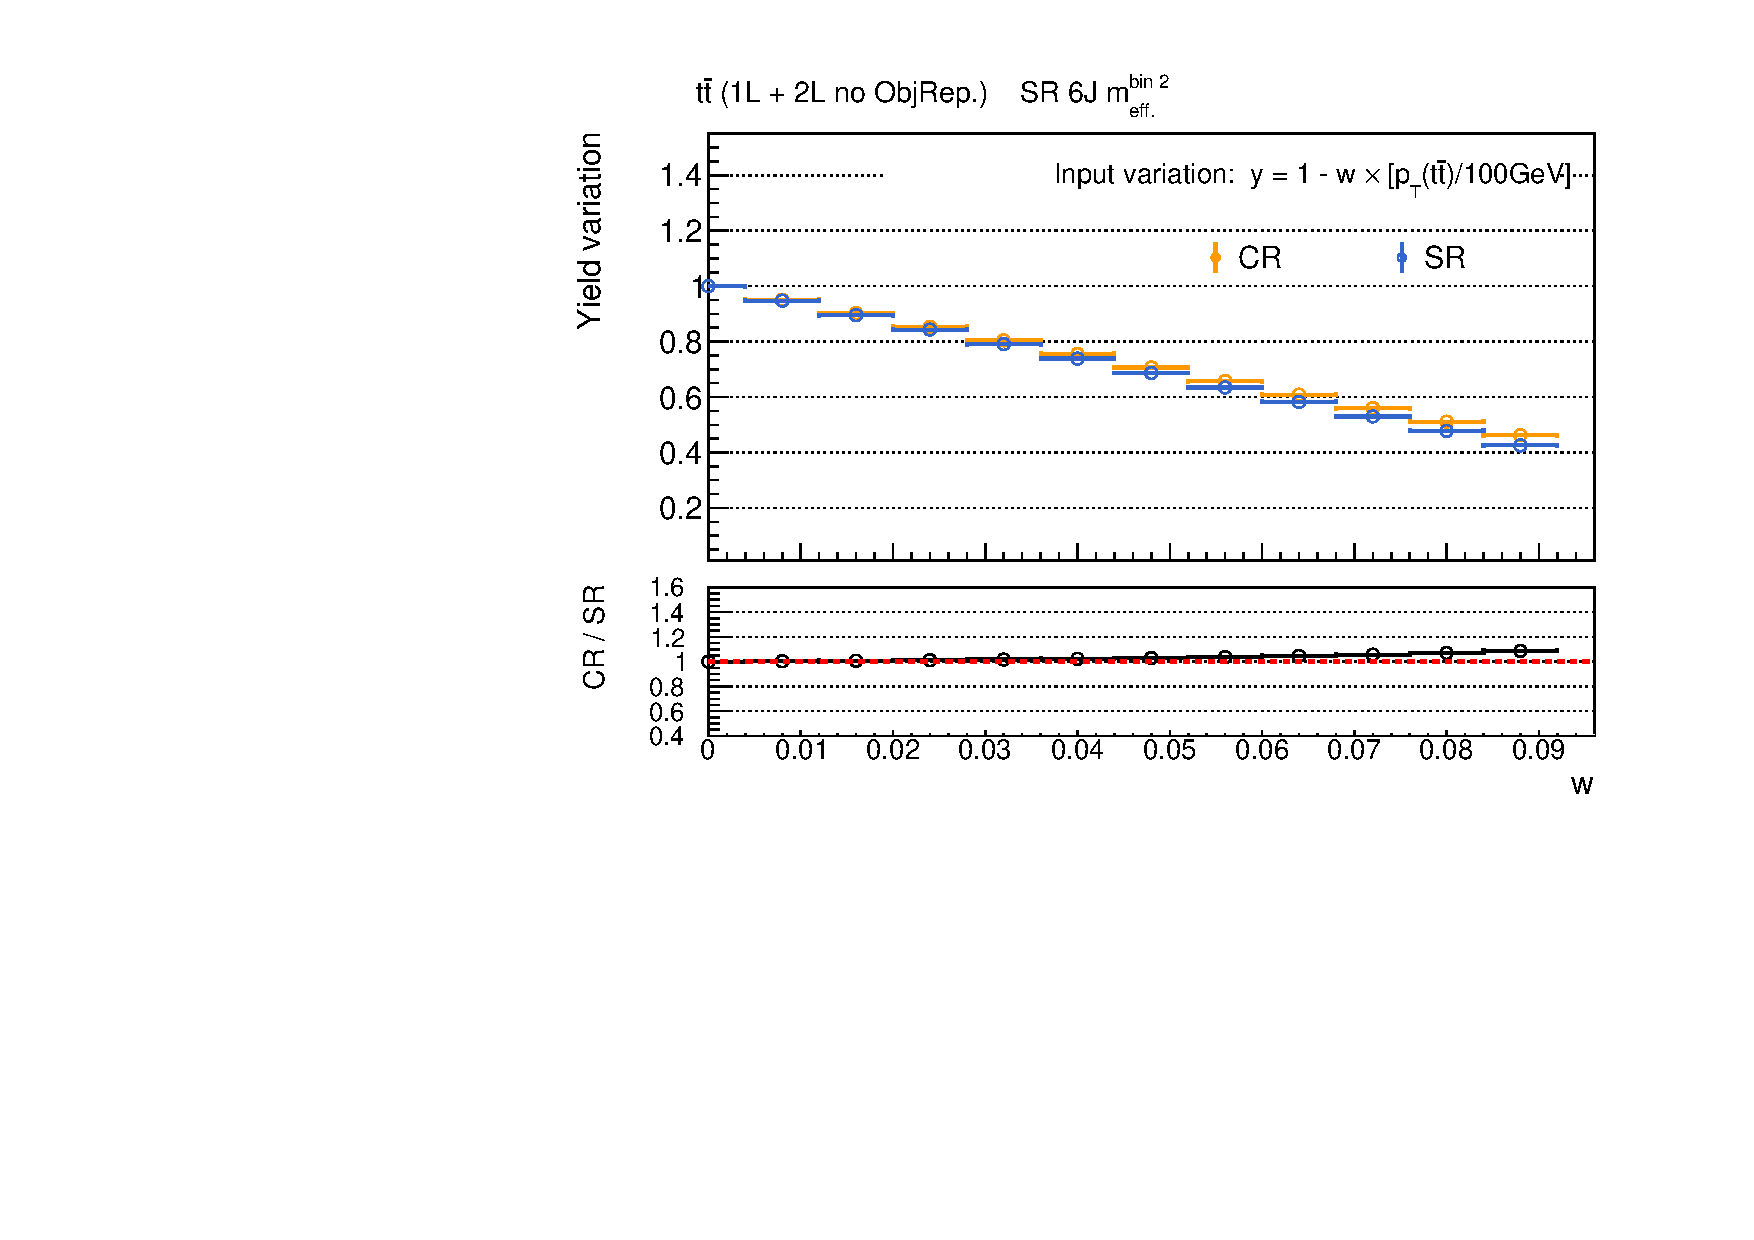
\includegraphics[width=0.488\textwidth]{figures/BGestimation/valid_extp/SFTF_ttNoObjRep_SR6JMEFF2_extp_var6J__ttPt.pdf}}
    \subfigure[]{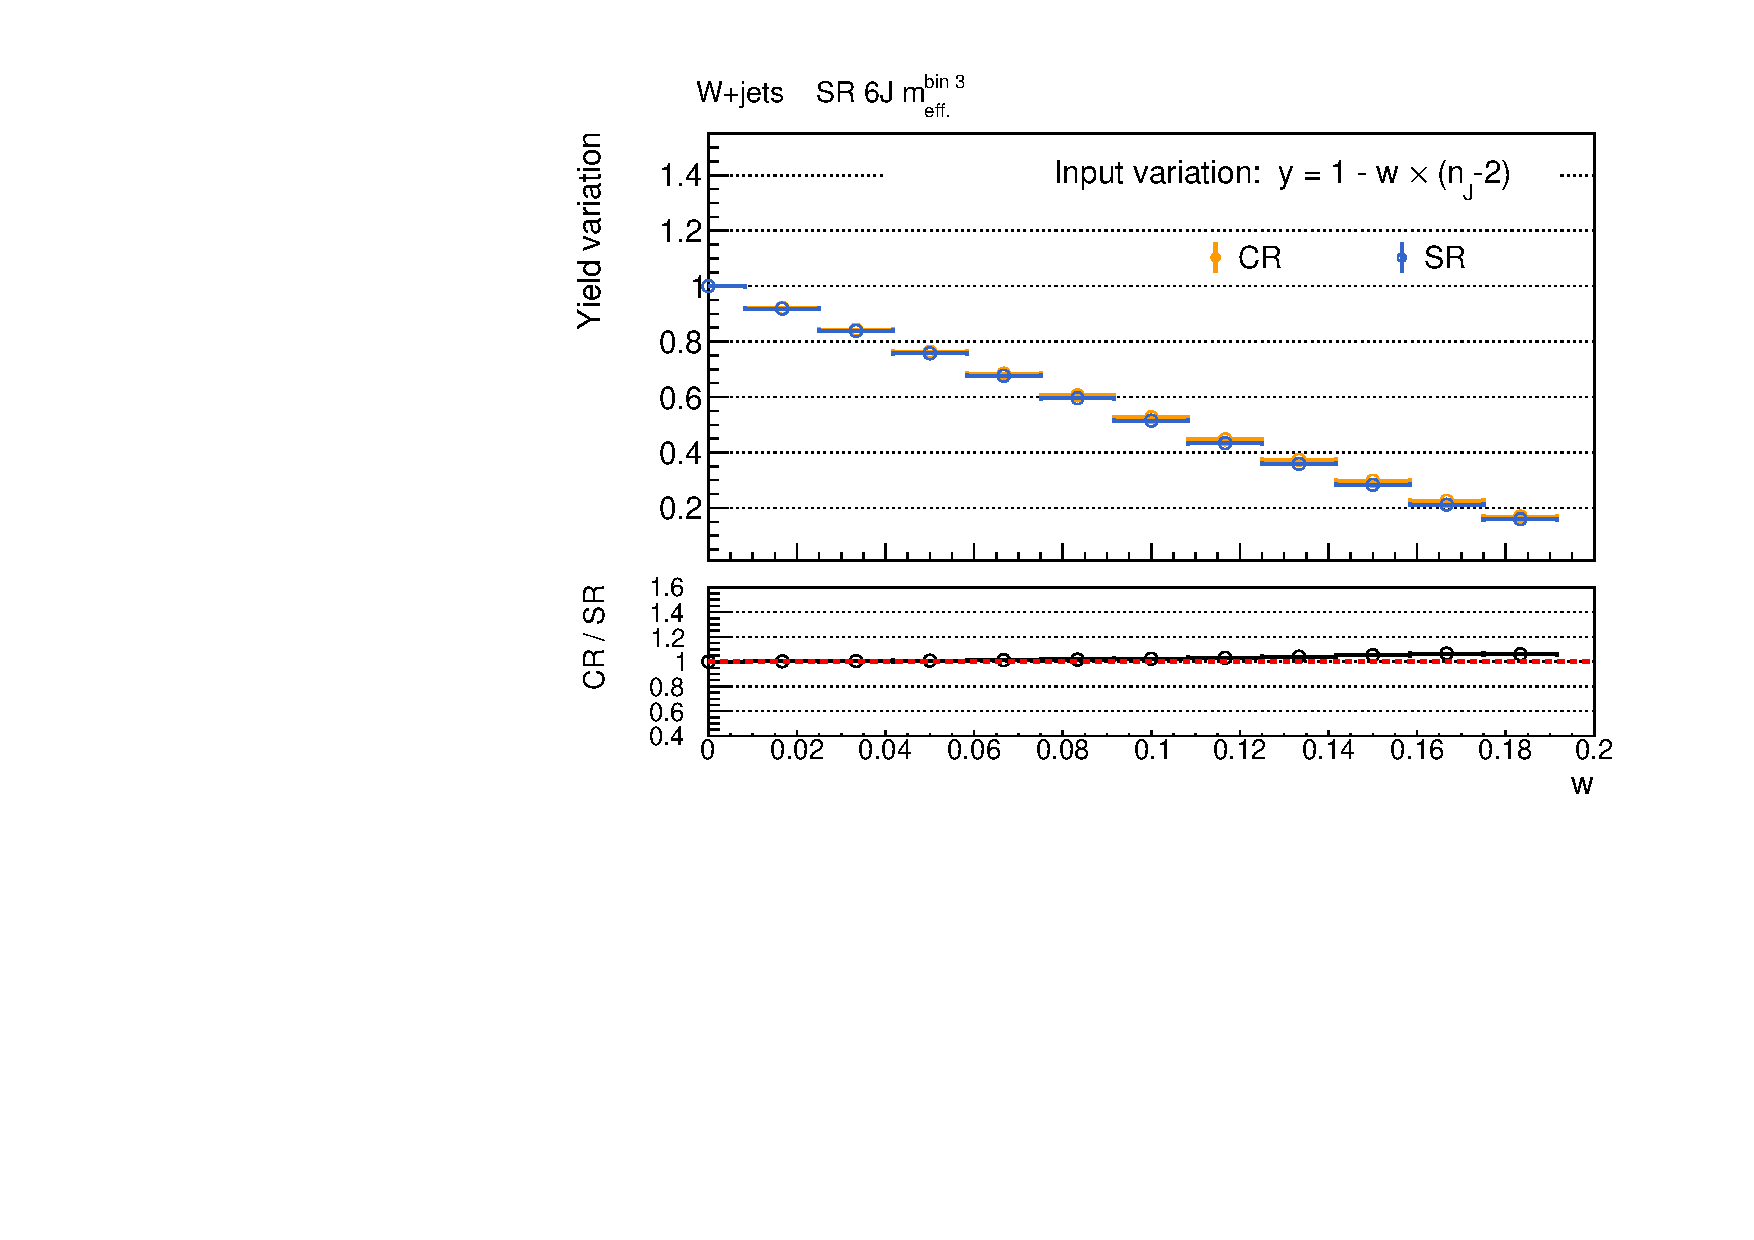
\includegraphics[width=0.488\textwidth]{figures/BGestimation/valid_extp/SFTF_wjets_SR6JMEFF3_extp_var6J__nJet30.pdf}}
    \subfigure[]{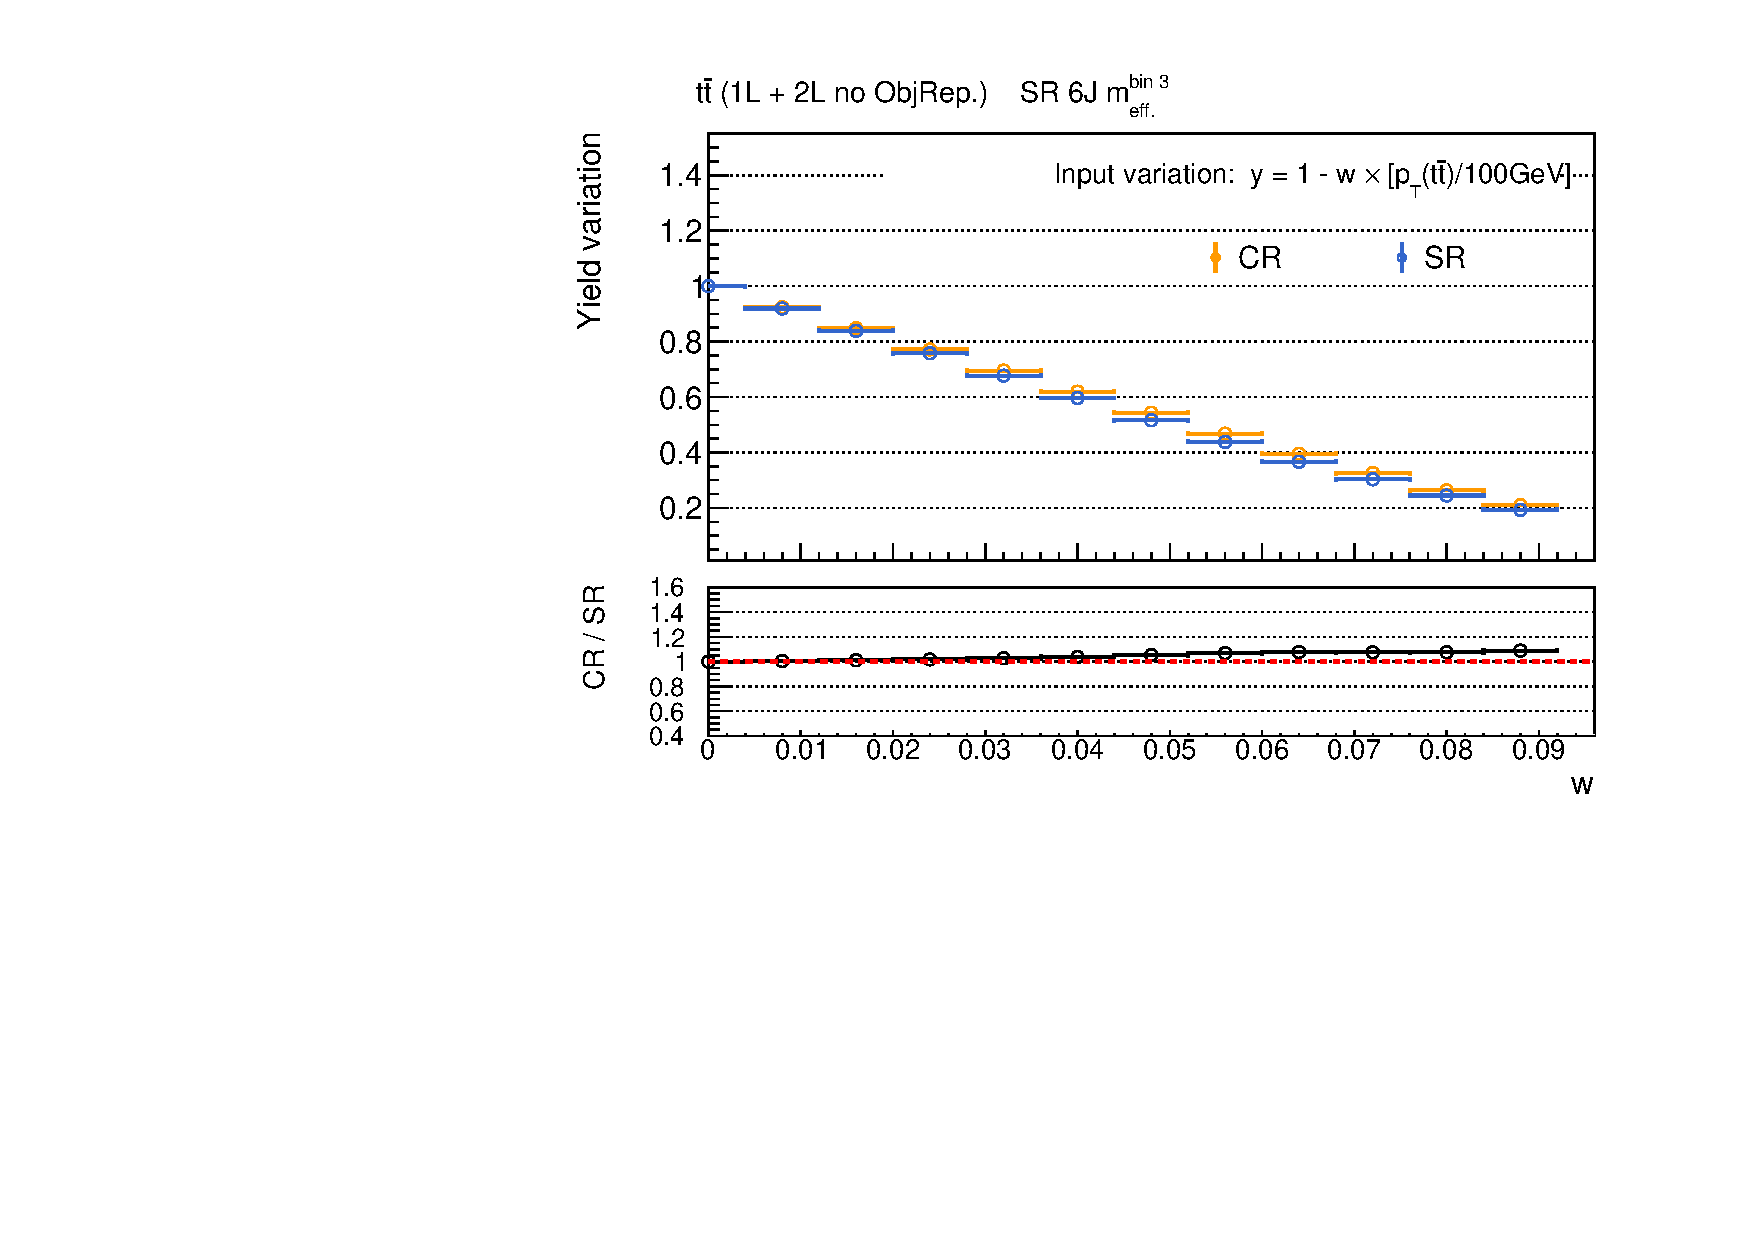
\includegraphics[width=0.488\textwidth]{figures/BGestimation/valid_extp/SFTF_ttNoObjRep_SR6JMEFF3_extp_var6J__ttPt.pdf}}
 \caption{Extrapolation error in SR/CR 6J. B-tagging requirement is removed. Top pannels show the yield variation of (a) $\wjets$ and (b) $\ttbar$ when injecting the variation by reweighting the MC with Eq. \ref{eq::BGestimation::injected_MCvariation}. Bottom rows are the relative difference in their response against the injected variation, namely the extrapolation errir. For the $\ttbar$ process, component estimated by the object replacement method is removed.  \label{fig::BGestimation::valid_extp_6J} }
\end{figure}


%%%%%%%%%%%%%%%% Lowx
\begin{figure}[h]
  \centering
    \subfigure[]{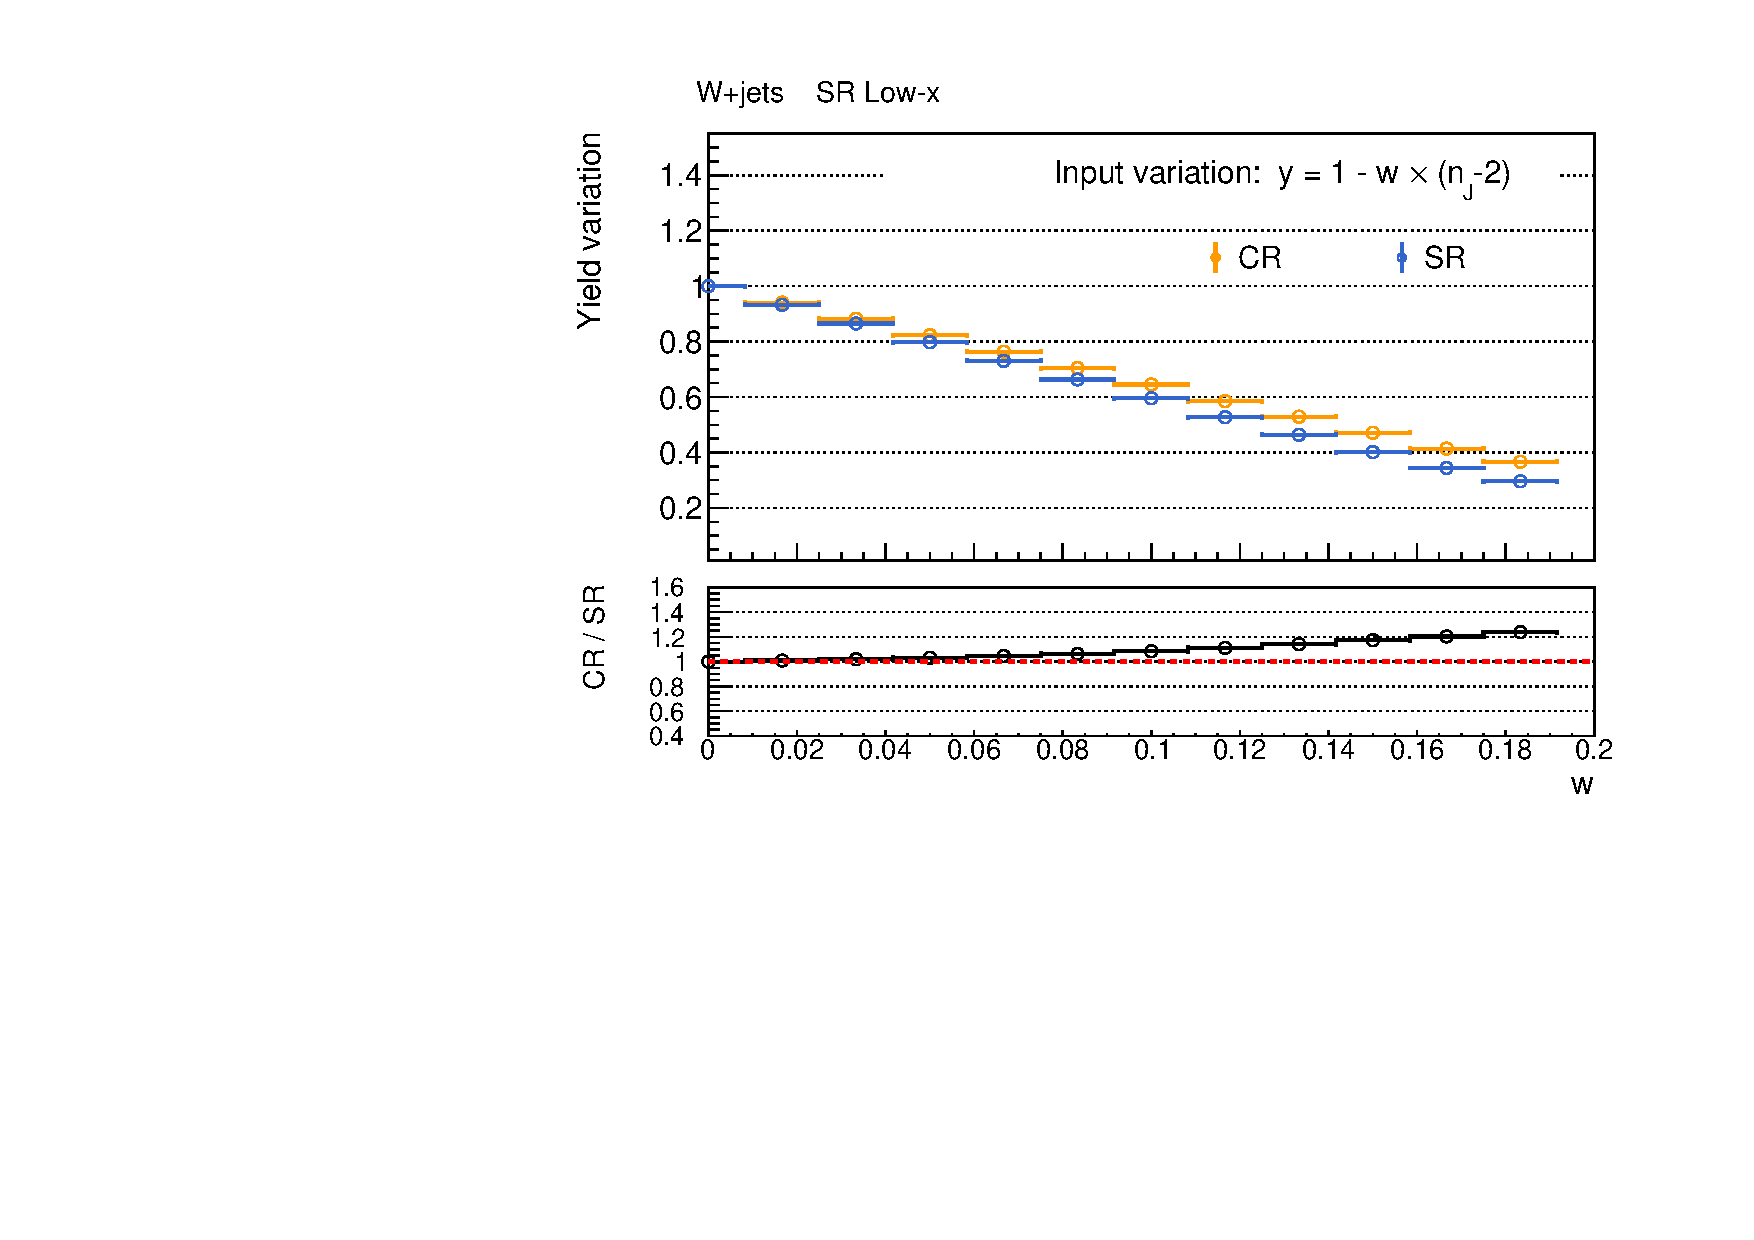
\includegraphics[width=0.488\textwidth]{figures/BGestimation/valid_extp/SFTF_wjets_SRLowx_extp_varLowx__nJet30.pdf}}
    \subfigure[]{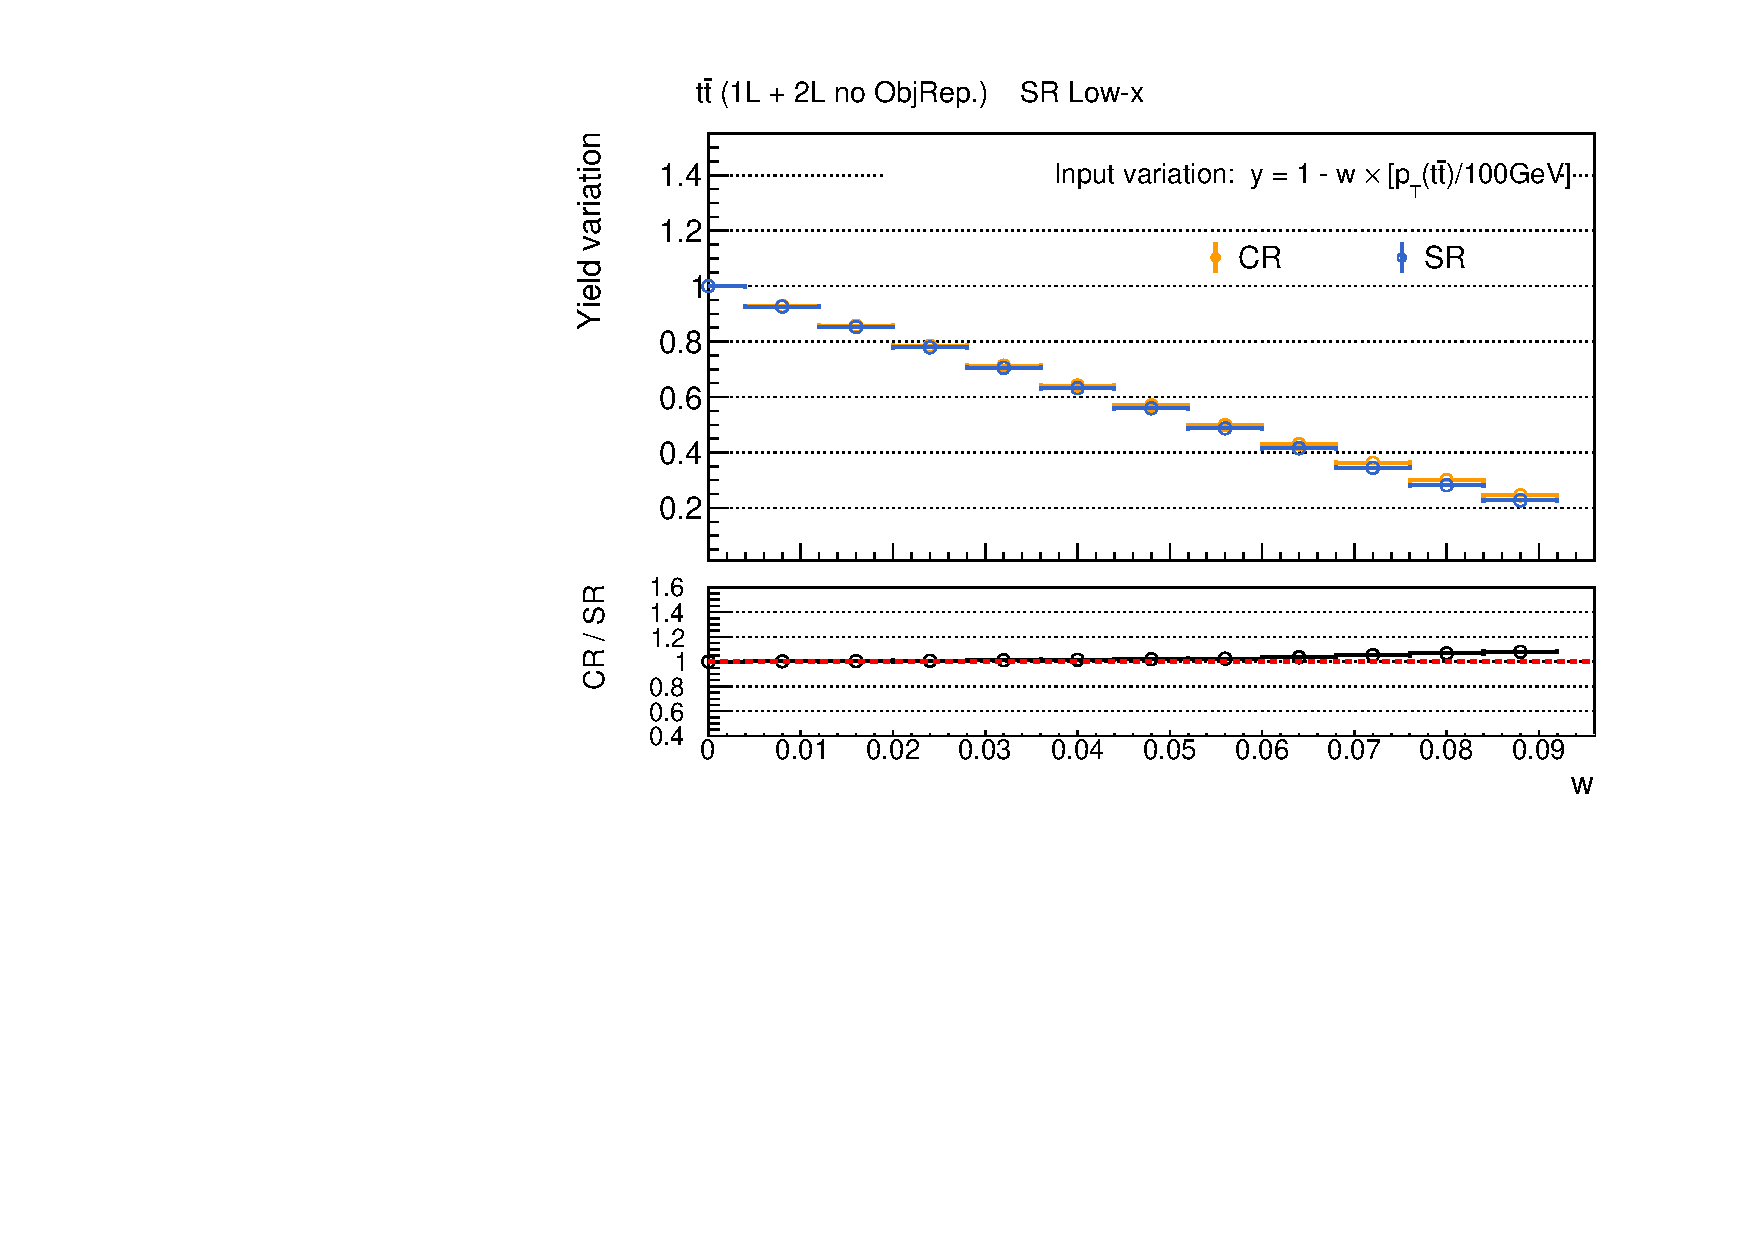
\includegraphics[width=0.488\textwidth]{figures/BGestimation/valid_extp/SFTF_ttNoObjRep_SRLowx_extp_varLowx__ttPt.pdf}}

%%%%%%%%%%%%%%%% Highx
    \subfigure[]{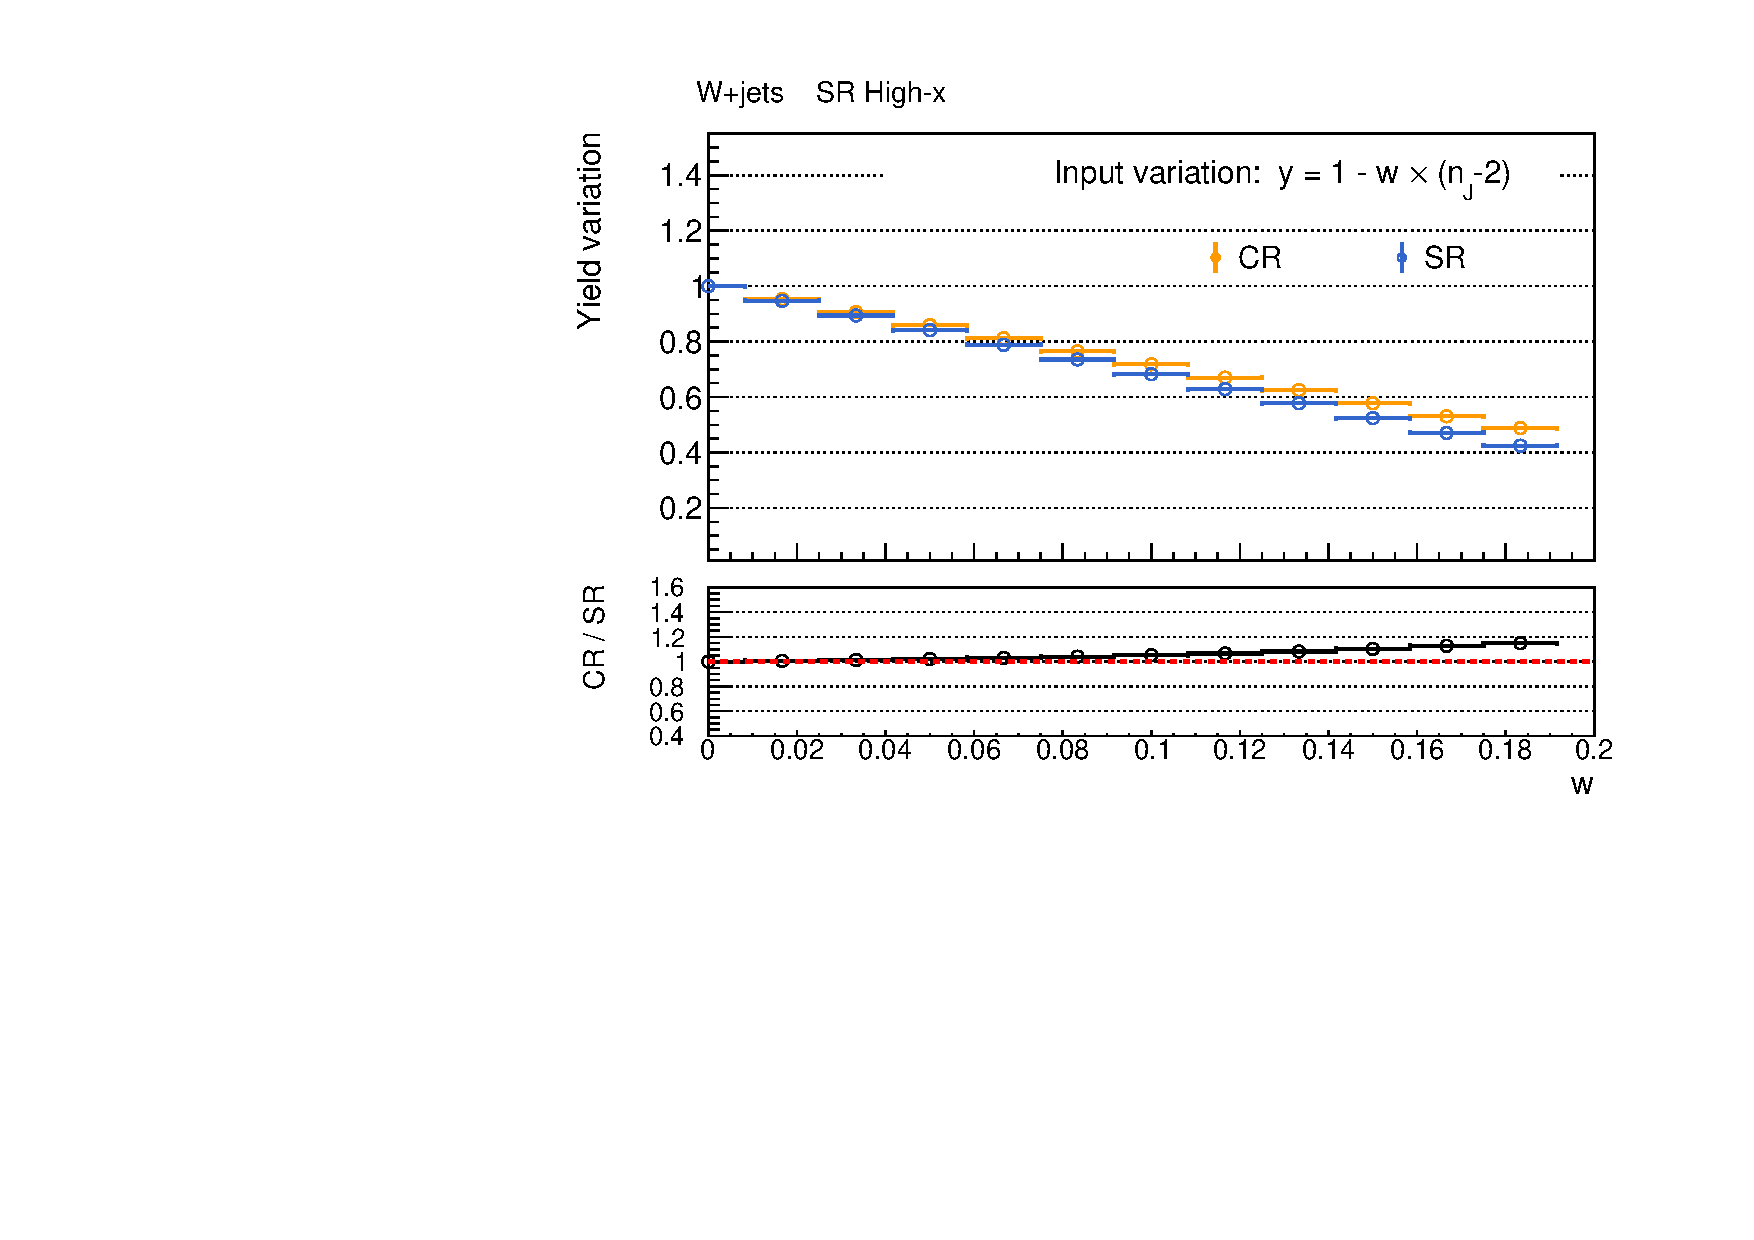
\includegraphics[width=0.488\textwidth]{figures/BGestimation/valid_extp/SFTF_wjets_SRHighx_extp_varHighx__nJet30.pdf}}
    \subfigure[]{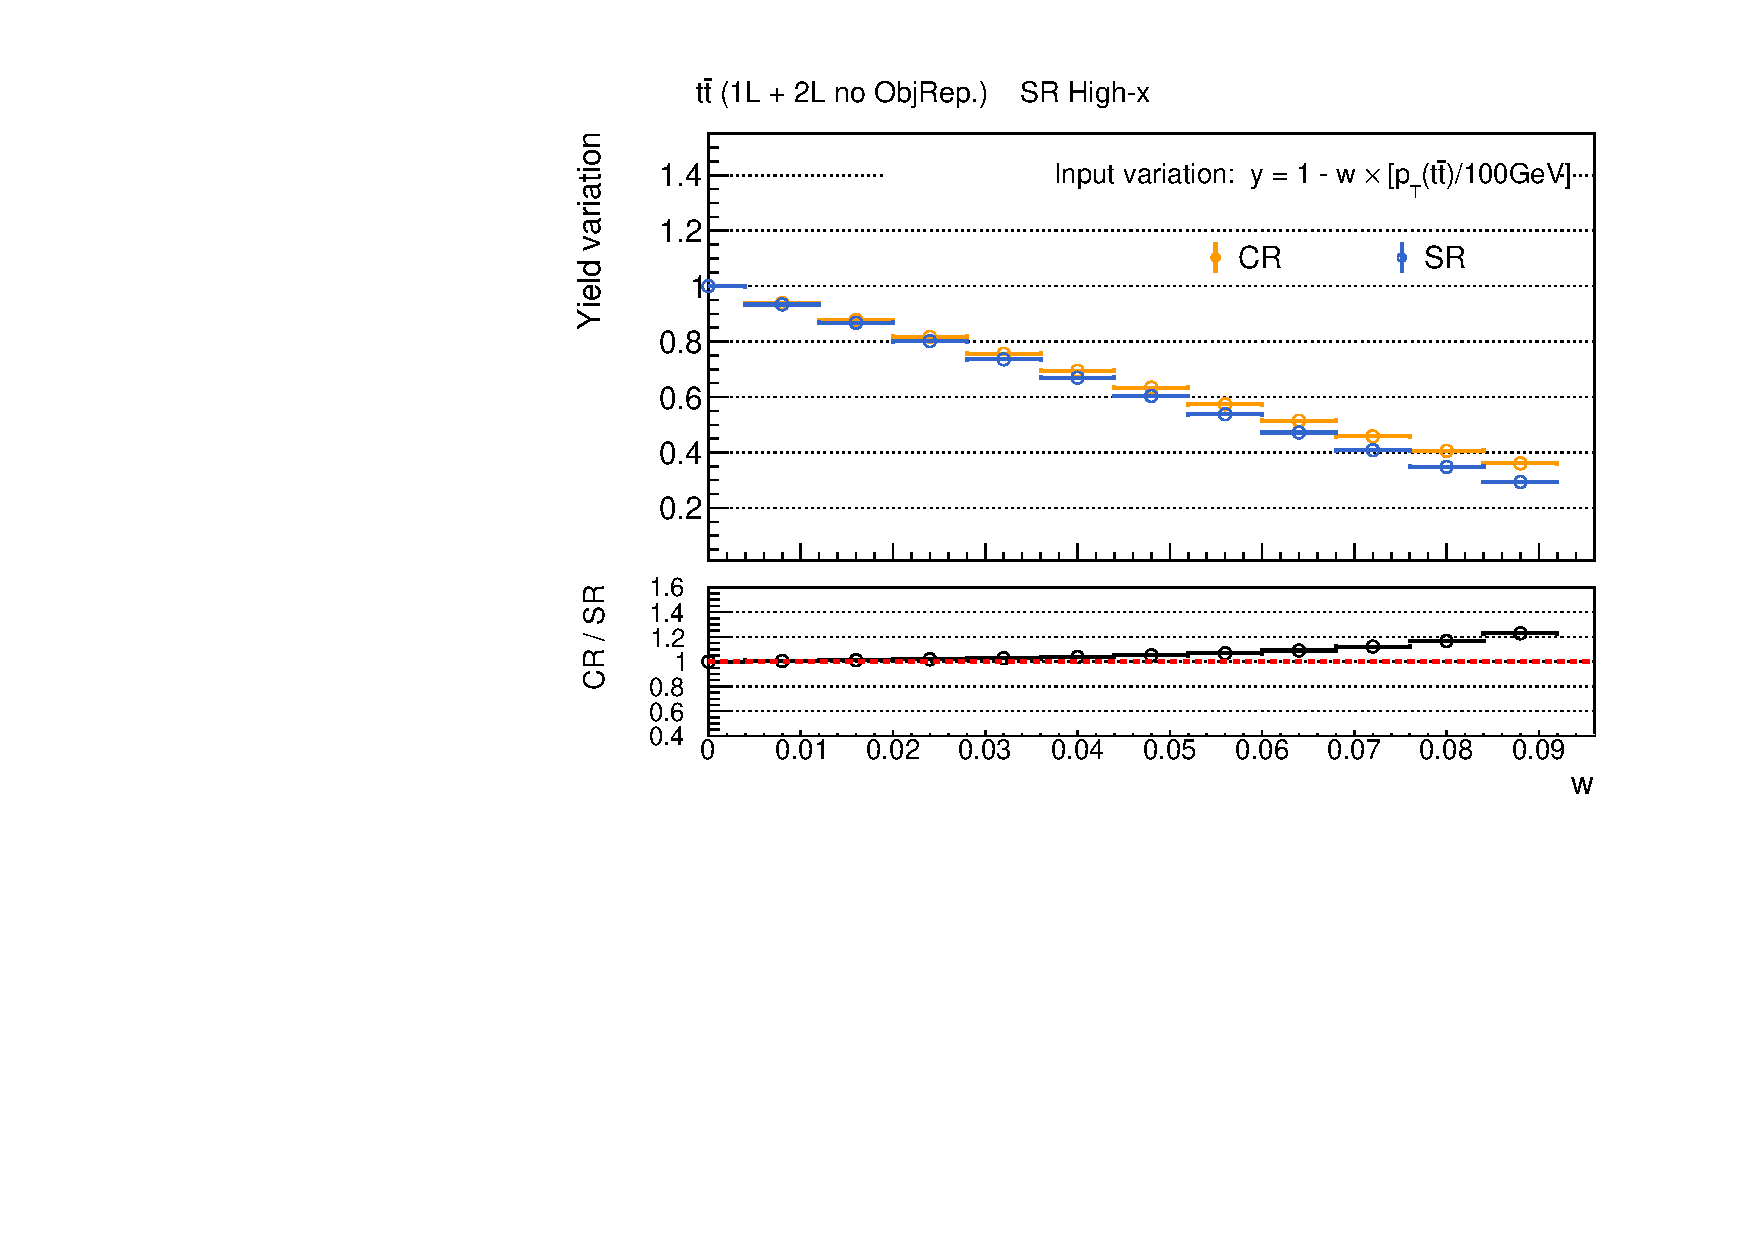
\includegraphics[width=0.488\textwidth]{figures/BGestimation/valid_extp/SFTF_ttNoObjRep_SRHighx_extp_varHighx__ttPt.pdf}}
 \caption{Extrapolation error in SR/CR (a)(b) Low-x, and (c)(d) High-x. B-tagging requirement is removed. Top pannels show the yield variation of $\wjets$ (left) and $\ttbar$ (right) when injecting the variation by reweighting the MC with Eq. \ref{eq::BGestimation::injected_MCvariation}. Bottom rows are the relative difference in their response against the injected variation, namely the extrapolation errir. For the $\ttbar$ process, component estimated by the object replacement method is removed.  \label{fig::BGestimation::valid_extp_6J} }
\end{figure}


%%%%%%%%%%%%%%%% 3B
\begin{figure}[h]
  \centering
    \subfigure[]{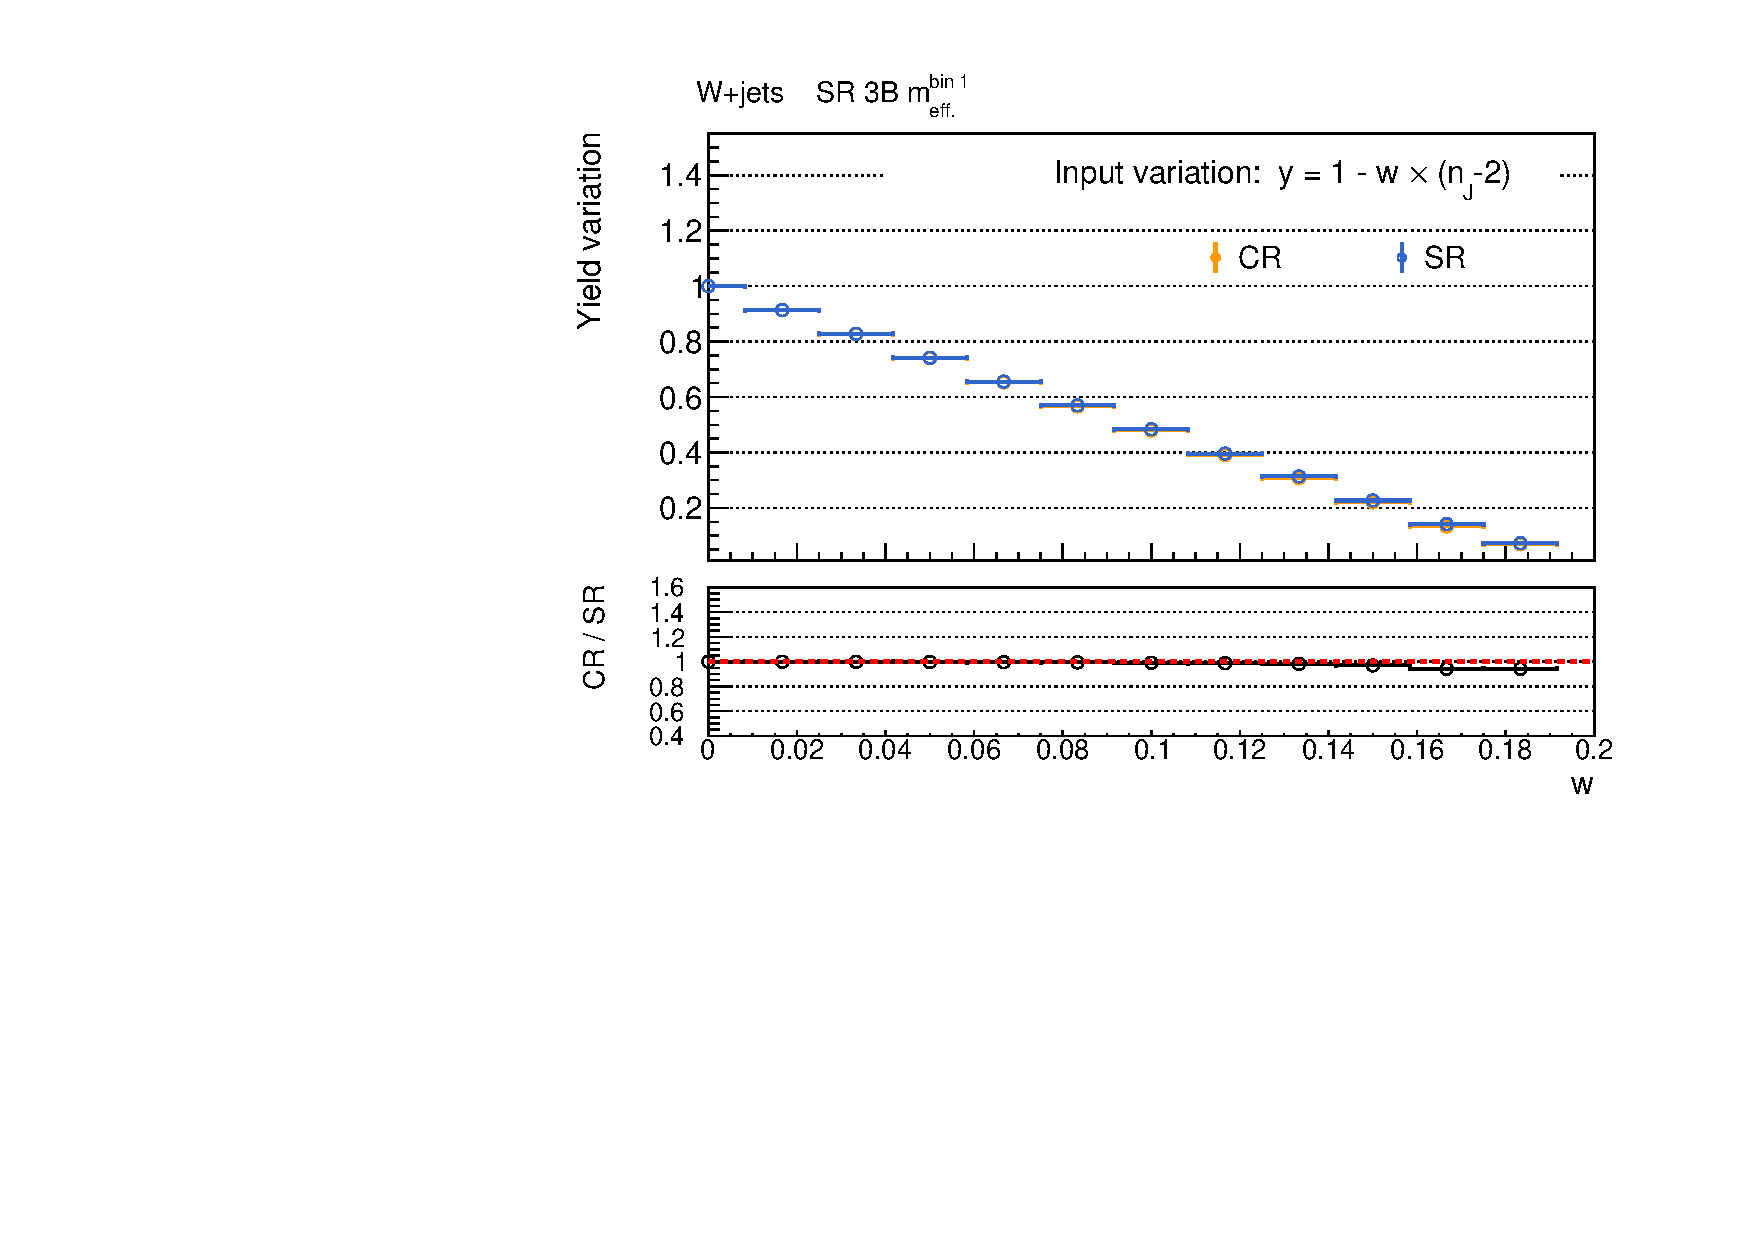
\includegraphics[width=0.488\textwidth]{figures/BGestimation/valid_extp/SFTF_wjets_SR3BMEFF1_extp_var3B__nJet30.pdf}}
    \subfigure[]{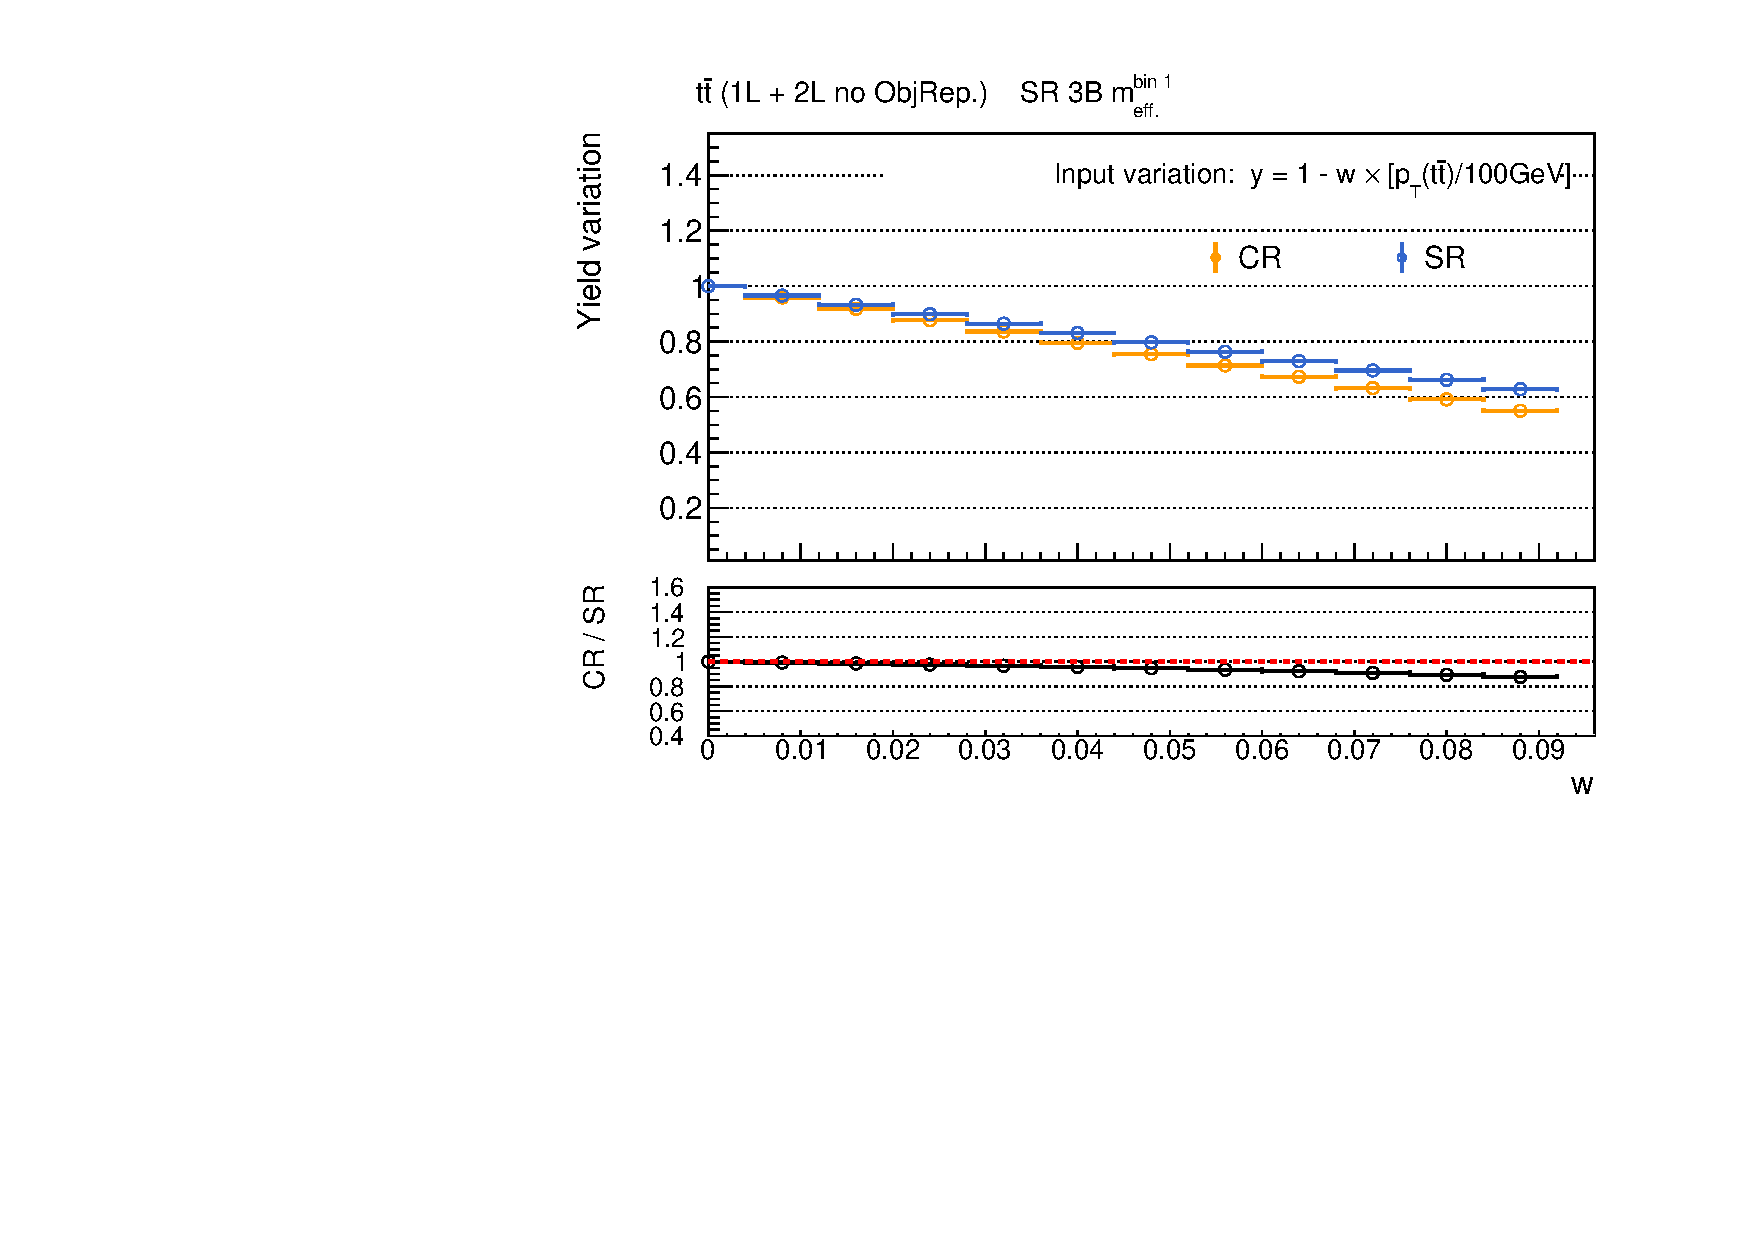
\includegraphics[width=0.488\textwidth]{figures/BGestimation/valid_extp/SFTF_ttNoObjRep_SR3BMEFF1_extp_var3B__ttPt.pdf}}
    \subfigure[]{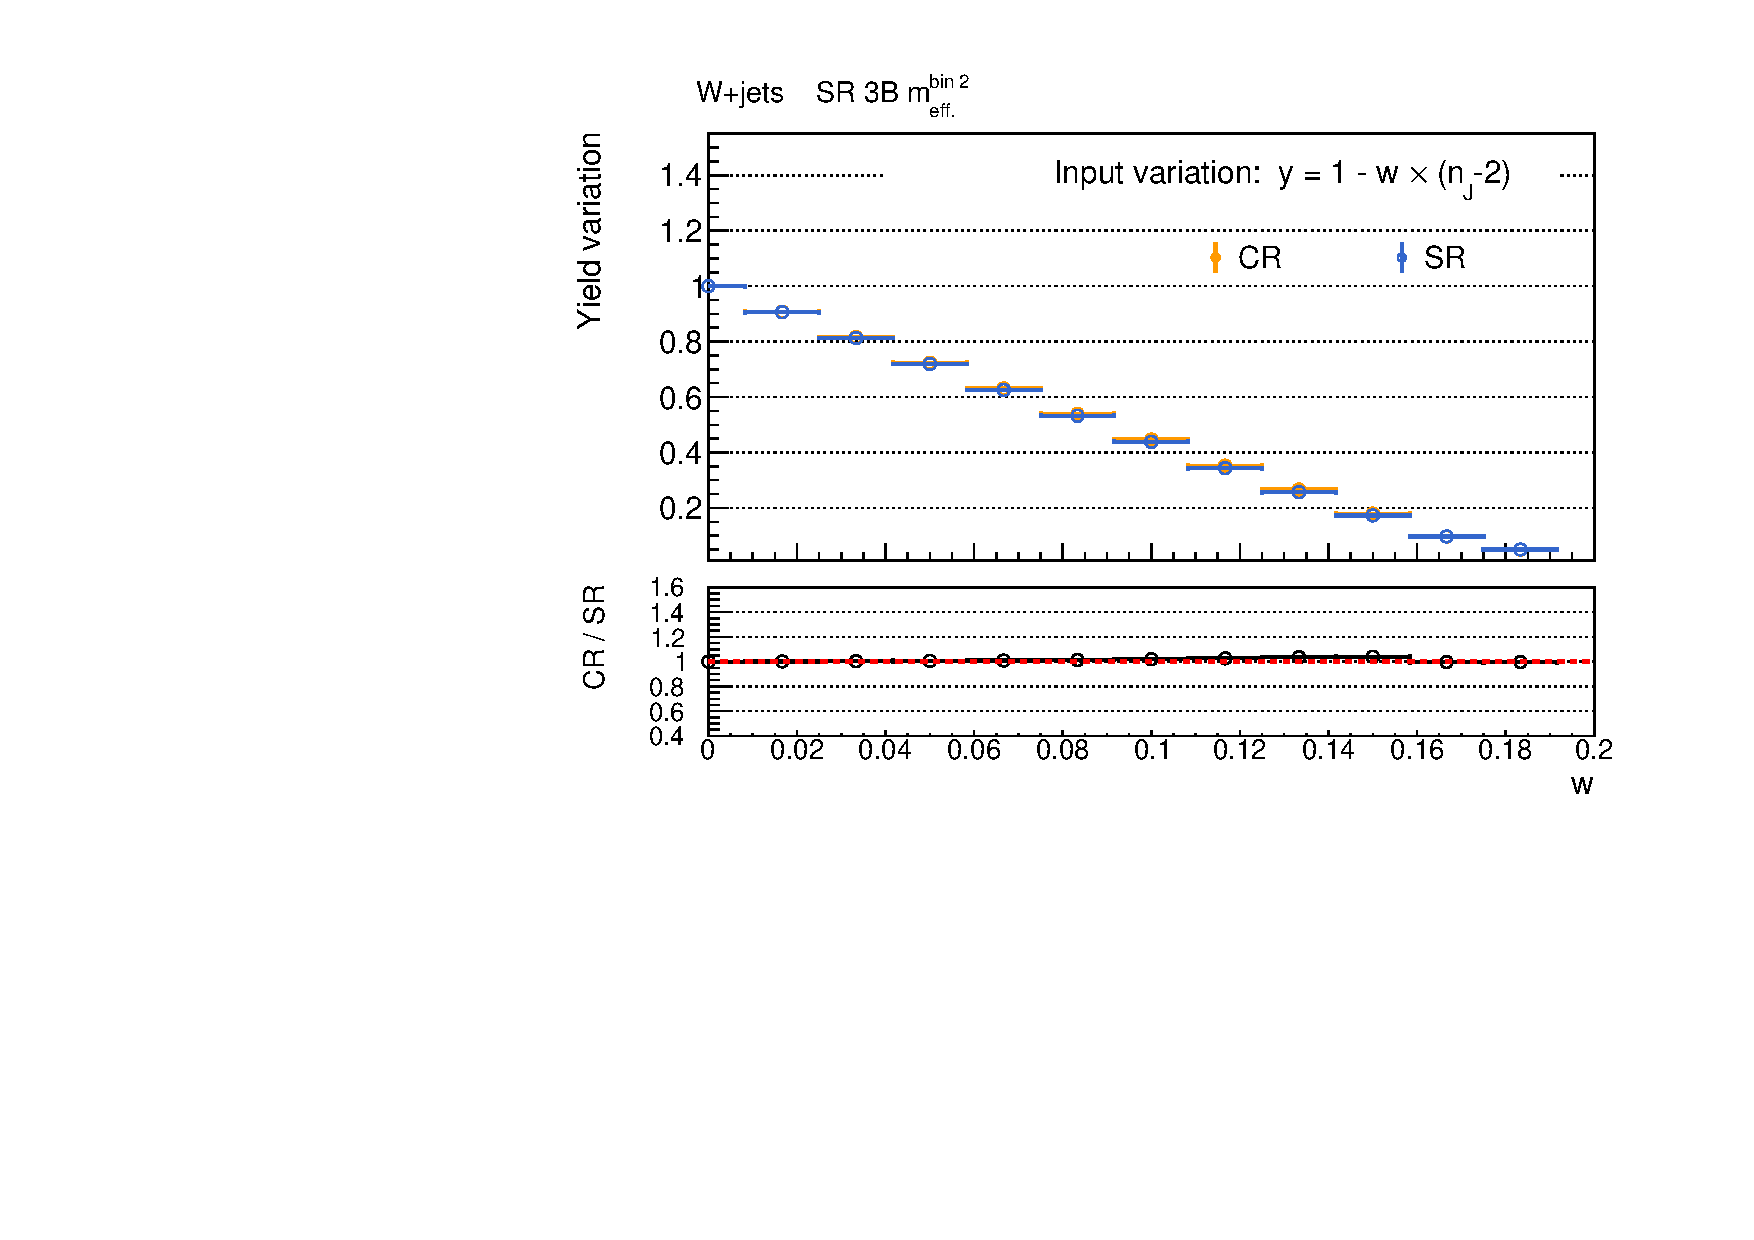
\includegraphics[width=0.488\textwidth]{figures/BGestimation/valid_extp/SFTF_wjets_SR3BMEFF2_extp_var3B__nJet30.pdf}}
    \subfigure[]{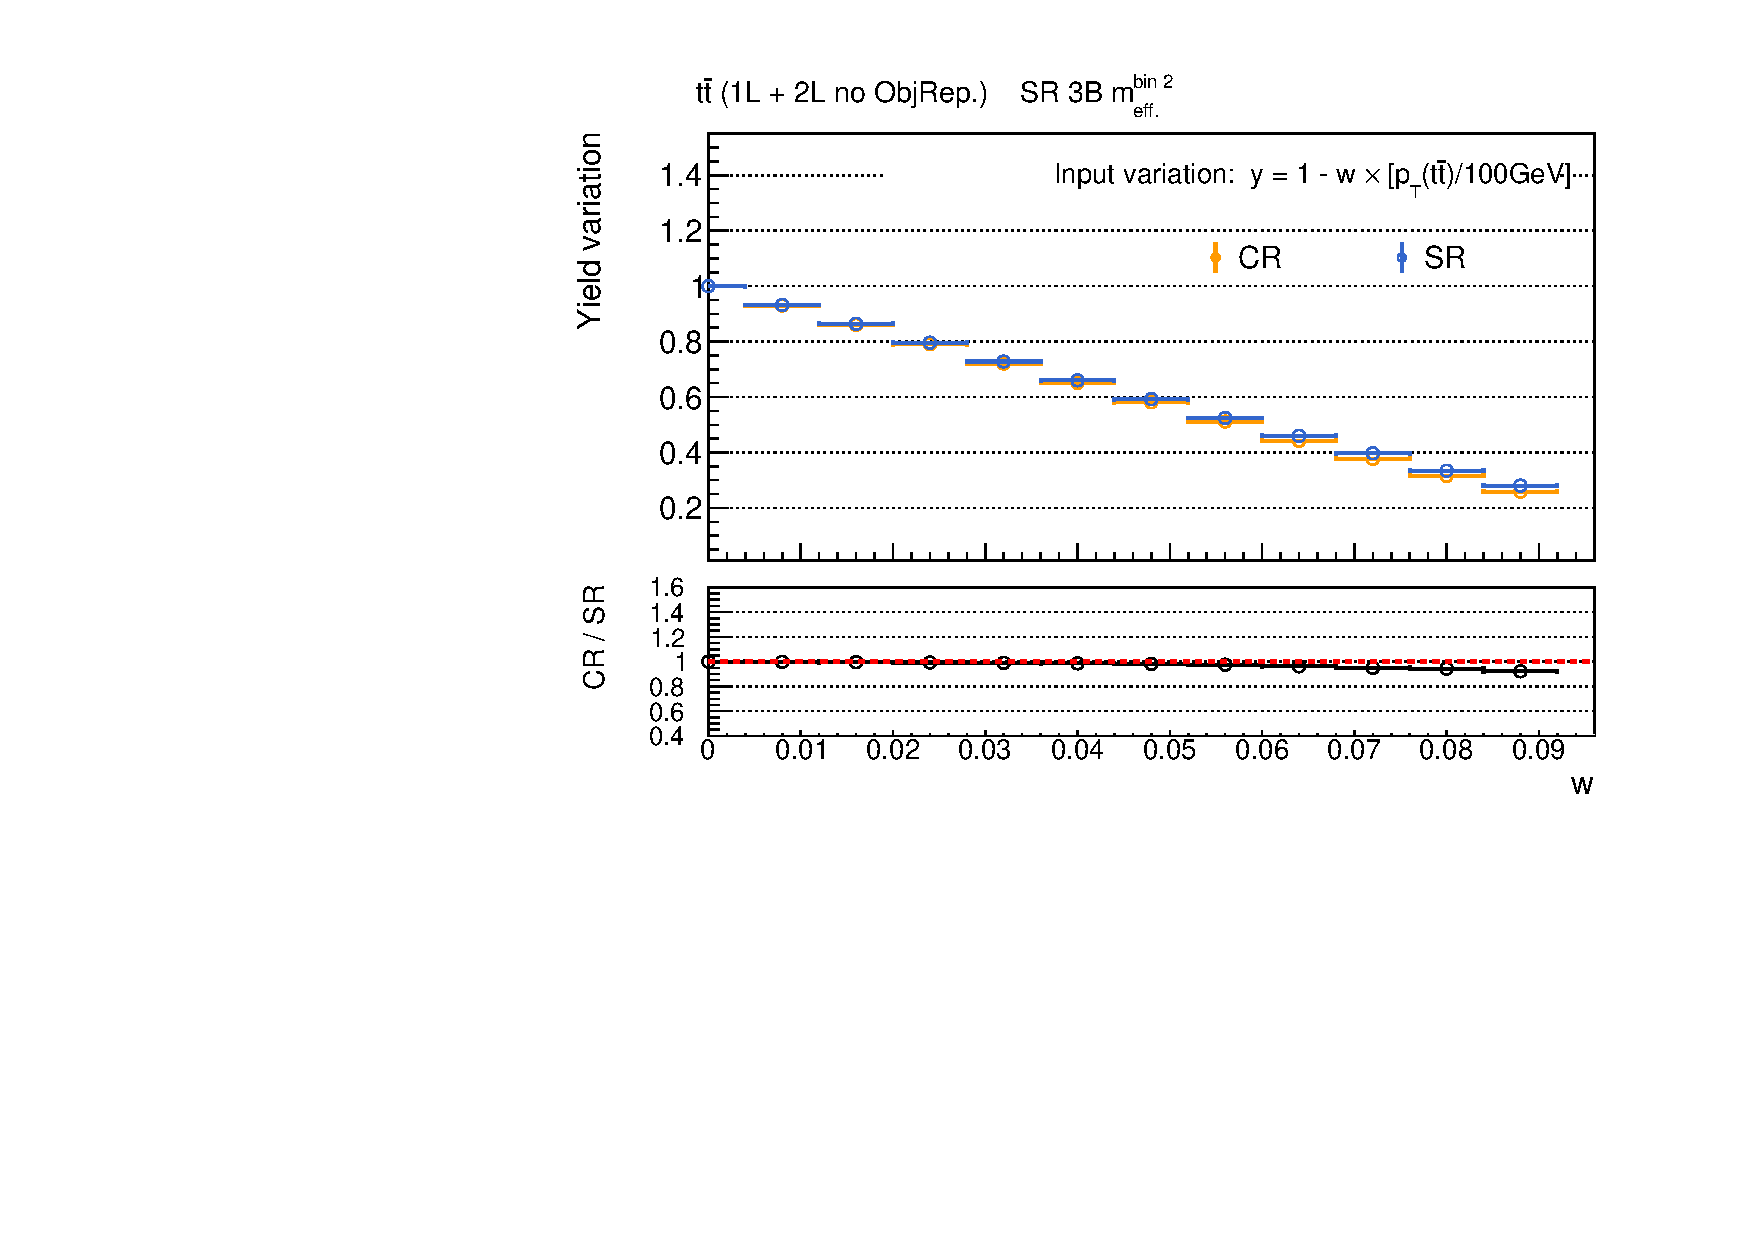
\includegraphics[width=0.488\textwidth]{figures/BGestimation/valid_extp/SFTF_ttNoObjRep_SR3BMEFF2_extp_var3B__ttPt.pdf}}
 \caption{Extrapolation error in SR/CR 3B. B-tagging requirement is removed for $\wjets$. Top pannels show the yield variation of $\wjets$ (left) and $\ttbar$ (right) when injecting the variation by reweighting the MC with Eq. \ref{eq::BGestimation::injected_MCvariation}. Bottom rows are the relative difference in their response against the injected variation, namely the extrapolation errir. For the $\ttbar$ process, component estimated by the object replacement method is removed.  \label{fig::BGestimation::valid_extp_3B} }
\end{figure}






